\documentclass[10pt, twocolumn, twoside]{article}
\usepackage[T1]{fontenc}
\usepackage{cuted}
\usepackage{graphicx}
\usepackage{bm}
\usepackage{geometry}
\usepackage{bbm}
\geometry{a4paper,total={170mm,257mm},left=17mm,top=20mm,right=17mm}
\usepackage{setspace}
\pagenumbering{arabic}
\usepackage{hyperref}
\usepackage{url}
\usepackage{scrextend}
\usepackage{amsmath,amssymb,amsthm}
\usepackage{ragged2e}
\usepackage{xcolor}
\usepackage{dirtytalk}
\usepackage{algorithm, algorithmic}
\usepackage{multicol}
\setcounter{tocdepth}{1}
\usepackage[backend=biber,style=nature,sorting=none]{biblatex}
\addbibresource{hubbardQMC_references.bib}

\title{Quantum Monte Carlo Simulations of the Hubbard model}
\author{Francisco Monteiro de Oliveira Brito}
\date{\today}
\setlength\columnsep{2em}

\makeatletter

\begin{document}

\begin{strip}
\vspace*{\dimexpr-\baselineskip-\stripsep\relax}
\centering
\maketitle
\vskip\baselineskip
\noindent%\makebox[\textwidth]{\rule{1.1\paperwidth}{0.4pt}}
\vskip\baselineskip
\justify

\onehalfspacing

\begin{abstract}\paragraph{}
The interactions between the electrons in a solid give rise to effects that arise specifically due to the many-body nature of the system. The Hubbard model is a minimal model that encapsulates electron correlations. It goes beyond the periodic ionic potential perturbation to the free electron gas or tight binding approaches, which lead to band theory. One obtains the Hubbard Hamiltonian by adding the simplest possible electron-electron interaction term to a tight binding Hamiltonian: an on-site interaction term that penalises double occupancy of a site. From it, we can make predictions about properties of a strongly correlated system, namely magnetic and superconducting behavior, and metal-insulator transitions. Quantum Monte Carlo (QMC) is a simulation method that is amply applicable to condensed matter physics problems and that is commonly used to simulate the Hubbard model. Despite the system size being constrained due to limited simulation time, the method provides reliable, unbiased, and generally accurate solutions to the often otherwise intractable quantum many-body problem. In particular, the technique allows us to capture the elusive effects of electron correlations, for example in two-dimensional graphene-like nanostructures.
\end{abstract}
\end{strip}

\section{Introduction}\paragraph{}
\onehalfspacing

The Hubbard model appeared in 1963 as one of the first attempts to include electron correlation effects in a quantum mechanical description of a solid \cite{Hubbard1963}. Originally, it was introduced to explain the behavior of the electrons occupying the narrow, partially filled $d-$bands of transition metals. Correlation phenomena in these bands lead to a behavior reminiscent of the atomic picture of a solid. We have come a long way since the introduction of the Hubbard model and it is now as paradigm-defining in many-body theory as the Ising model in statistical physics\cite{Mahan2000}.

These notes aim to present the basic aspects of a numerical technique used to simulate the Hubbard model in a self-contained, tutorial form. The idea is to reduce our problem to solving a set of integrals, which we evaluate numerically through a standard stochastic procedure, known as the Monte Carlo method. These integrals are arrived at upon formulating the quantum many-body description of the system using the Schr\"odinger equation. Hence the name Quantum Monte Carlo, which is used to distinguish it from Classical Monte Carlo. In the classical version, one measures thermal averages. In the quantum version, one measures expectations of operators over the Hilbert space of the system, corresponding to physical observables that fluctuate with a dynamics given by Schr\"odinger's equation.

When Hubbard's seminal paper came out, it followed a trend that arose in the 1950's when people were working on a theory of correlation effects in the free electron gas \cite{Bohm1953, Gell-Mann1957, Sawada1957, Hubbard1957, Hubbard1958, Nozieres1958}. Hubbard devised a simple model for the seemingly intractable problem of interacting electrons in a band. His work explained qualitatively some properties of transition and rare-earth metals in which electron correlations are non negligible. It turns out that the mathematical formulation of the interaction problem for correlated electrons in a band is not prohibitively complicated, and is amenable to both analytical and numerical computations after some reasonable approximations are introduced. Notably, the model is particularly adapted to computer simulations because of its simple approximate Hamiltonian. Moreover, it has been shown to be very relevant in the description of Mott insulators, and high $T_c$ superconductors. In fact, the Hubbard model has found many applications, describing successfully a variety of quantum systems\cite{Editorial2013}; nonetheless, even the simplified picture it offers is in general difficult to approach analytically. There exists an exact solution in one dimension via Bethe ansatz\cite{Lieb1968}, but the more general higher dimensional case is often solved numerically. An example of particular relevance here is the study carried out by Hirsch \cite{Hirsch1985}. In what follows we will discuss how to simulate the Hubbard model using a similar numerical approach.

An example of an application of a QMC technique is the simulation of electron correlations in a transition metal dichalcogenide (TMD) nanoribbon, a two-dimensional nanostructure made out of some graphene-like compound \cite{Yang2017, Raczkowski2017, Chen2017, Wang2012, Braz2017}. The structure is much longer on one direction than on the other, resembling a ribbon, hence its name. The electronic states that accumulate on the edges of this ribbon might lead to interesting magnetic behavior in these TMD nanostructures (as they do in the analogous graphene nanostructures\cite{Yazyev2010}) and this possibility remains unexplored numerically\cite{Feldner2011, Golor2013}. Moreover, there is some interest in exploring the phase diagram of these systems because recent studies point at the possibility of topological superconductivity \cite{Hsu2017}.

\section{Hubbard model}\paragraph{}

We start with an overview of the Hubbard model and in section \ref{hubbQMC} we provide details on how to simulate it numerically using quantum Monte Carlo. In particular, we discuss the original motivation to introduce the model and show how the Hubbard Hamiltonian arises as an approximate representation of the Coulomb repulsion between electrons. Finally, we present exact solutions for particular limiting cases, which can be used to crosscheck our simulations.

The nearly free electron gas models the conduction bands of metals and alloys fairly accurately. The high mobility of the electrons compared to the ions justifies two equivalent approximations, both giving essentially the same results\cite{Ashcroft1976}. The first idea is to treat the periodic potential created by the \emph{virtually} fixed ions (compared to the electrons) as a perturbation on the free electron gas. The other way of arriving at similar results is to imagine the system as a collection of tightly bond atoms, in which the higher energy conduction electrons hop from atom to atom. Both these approaches lead to band theory, a framework which allows us to predict whether a material is a conductor or a insulator. From the tight binding point of view, the effect of the electron mobility is the broadening of the atomic energy levels: the electrons in the solid occupy energy bands, rather than levels. The partially filled band of highest energy is called the conduction band, since it is the band occupied by conduction electrons hopping from atom to atom. However, in transition and rare-earth metals, there are partially filled bands other than to the conduction bands: $d-$ or $f-$bands. The partial filling of these bands and the electron correlations within them are responsible for the characteristic properties of these solids. Some of these properties are not explained by band theory, namely the Mott metal-insulator transition\cite{Boer1937, Mott1939, Mott1949}

Take Molybdenum, a transition metal. Its electronic configuration is $[Kr] 5s^1 4d^5$. The $s$-orbital is higher in energy than the $d$-orbital. Thus, the Fermi energy lies in the corresponding partially filled $s-$band, which is then the conduction band. However, the $d$-band will be only partially filled as well, leading to the effects mentioned in the previous paragraph. Platinum is yet another example, with electronic configuration $[Xe]4f^{14} 5d^9 6s^1 $, where the $5d$ level in only partially filled. In these partially filled narrow energy bands correlation phenomena are particularly relevant, as opposed to the case of conduction bands. Thus, the nearly free electron gas model does not suffice to describe the electrons in these bands; we must turn to a model that includes correlations. While for $f-$electrons of rare earth metals, a purely atomic, localized model - such as the Heitler-London model - might be satisfactory, the same cannot be said for $d-$electrons of transition metals because the band they occupy is narrower and correlations should be more relevant since the electronic states within the band are closer in energy.

\subsection{Electron correlations in narrow $d-$bands}\paragraph{}

First, note that the effects of correlations cannot possibly be the same in narrow energy bands and in the free electron gas. To see this, we may simply recall the shape of a $d-$wave function. In a $d-$orbital, the electron charge density is concentrated near the nucleus. In a solid the electronic charge density should then also be concentrated near the nuclei, as long as the atomic description is useful, even if not completely correct\footnote{The electronic charge density is, of course, not actually defined in terms of a squared norm of the $d-$wave function for a narrow band. There is some broadening of the corresponding atomic energy level, and the wave function describing an electron is a Bloch wave function. Since the band is narrow, we assume that the atomic wave function description is still somewhat useful in a given range and we use it to provide a heuristic motivation for the non validity of the free electron assumption.}. It is much smaller between atoms so that electrons do seem to belong to individual atoms in some sense. For a $d-$band, we assume that the case is not so different since the band is narrow. The fact that we may speak with some meaning of an electron belonging to a particular atom motivates an atomic description, in spite of the fact that the bandwidth of a $d-$band is still appreciable. The point is that electrons in $d-$bands are certainly not well described by a free electron gas, which cannot possibly account for atomic-like behavior.

\begin{figure}[ht!]\label{fig:hydrogenWF}
\centering
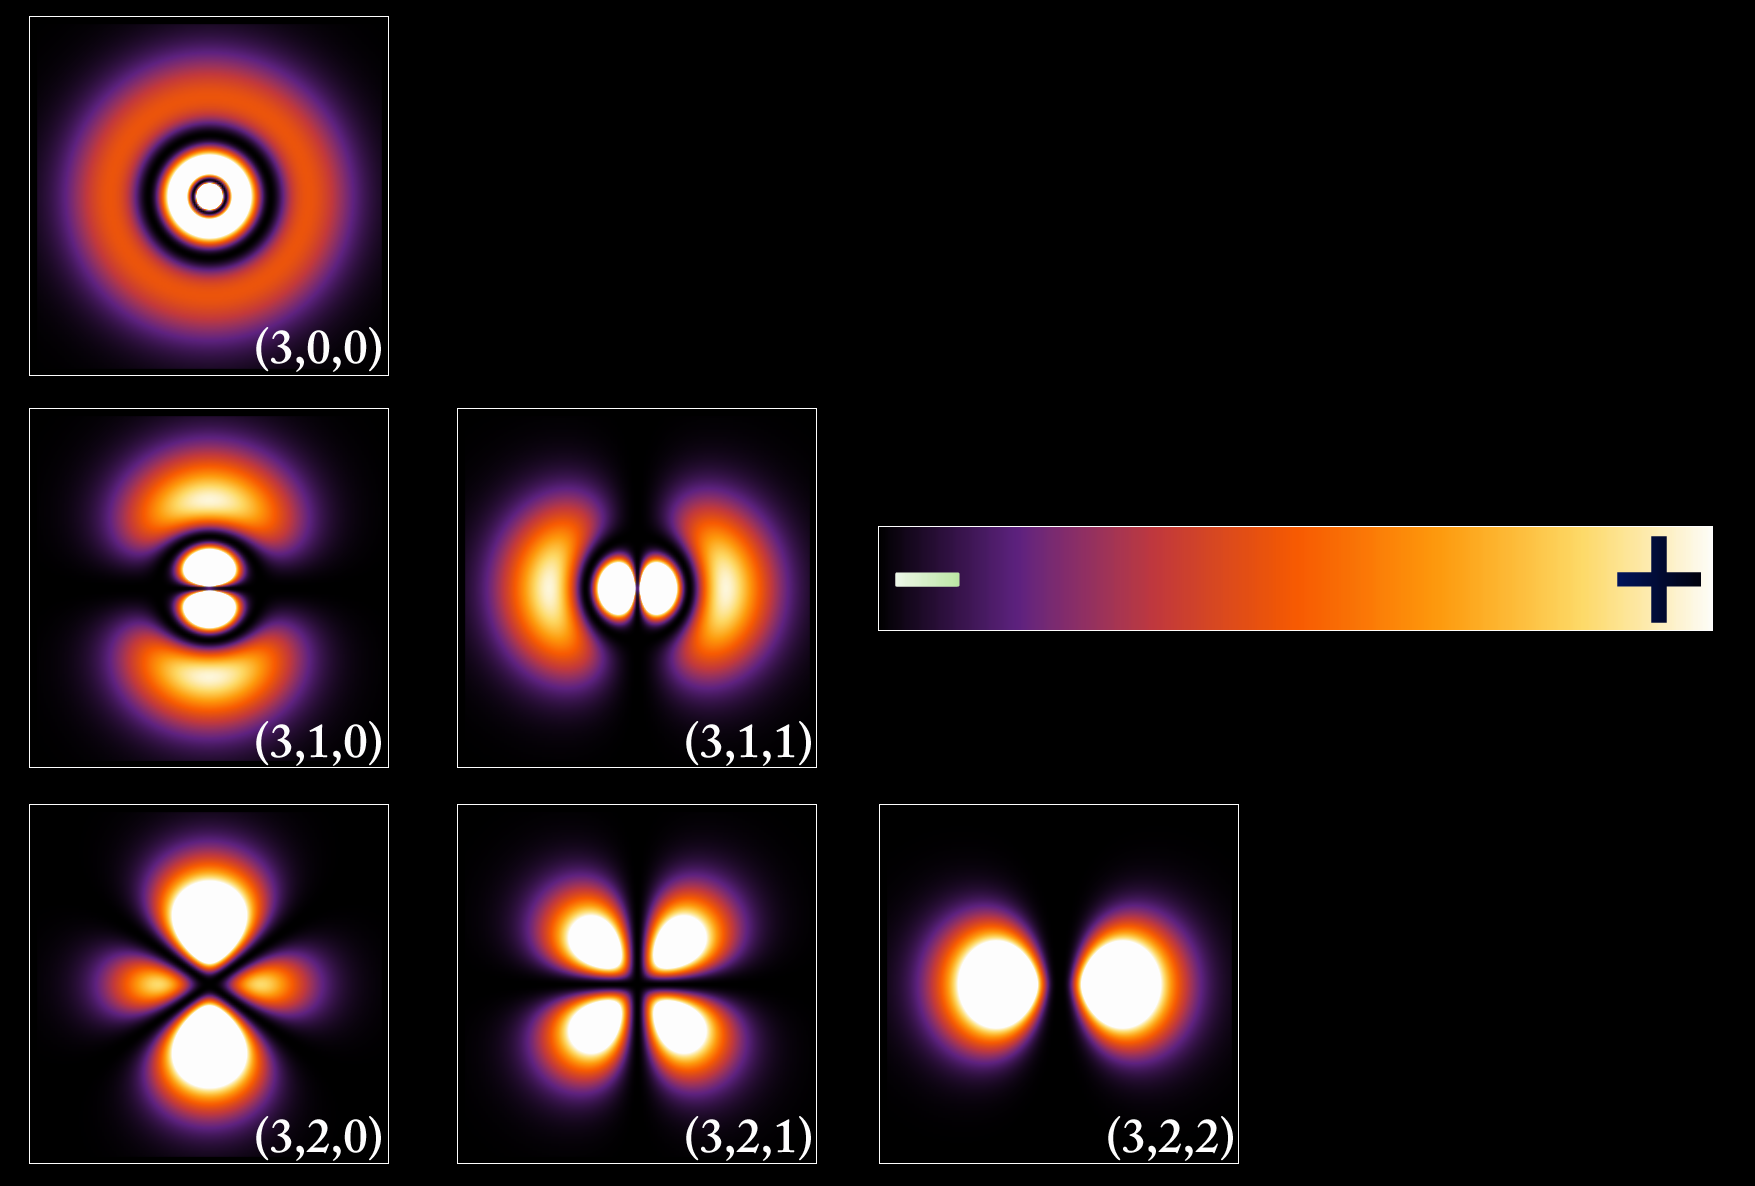
\includegraphics[width = 8.2cm]{Hydrogen_Density_Plots.png}
\caption{Probability density plots for different hydrogen orbital wave functions corresponding to quantum numbers $(n, l, m)$ for $n = 3$. d-wave functions correspond to $l=2$. Note that the probability density is always higher in a region near the nucleus, and has a complicated shape, which will lead to a non-uniform distribution of electronic charge, as opposed to the case of the free electron gas.}
\end{figure}

Experimentally, $d-$electrons of transition metals show a hybrid behavior: sometimes they are accurately described by an ordinary band model, but there are occasions in which the atomic model is better. For example, we see spin wave phenomena in ferromagnetic transition metals, and the susceptibilities of some of these metals depend strongly on temperature. This is characteristic of an atomic (Heisenberg) model. On the other hand, the $d-$electrons contribute significantly to the low temperature specific heat and sometimes the magnetic moments per atom of some transition metal ferromagnets are not integer multiples of the Bohr magneton. This is characteristic of band theory\footnote{Think, for example, of a tight binding model. Electrons hop from atom to atom, and in general the spin of each atom depends on the particular electrons \say{belonging} to it at a given time. If we take an average of the total spin of each atom, we will in general not necessarily obtain an integer multiple of the Bohr magneton. If we simply had a collection of atoms, Hund's rule would apply, and each atom would have its spin aligned in a given direction. The average spin would then tend to be an integer multiple of the Bohr magneton.}. Our theory of correlations should describe this balance between band-like and atomic-like behavior.

The atomic picture of a solid consists of an electron gas where ions are immersed. The ions then interact in much the same way as they do in salts. This extreme scenario is surely not even close to the true state of affairs since the number of $d-$electrons per atom is in general not an integer. This motivates us to introduce a less restrictive model, which is not too far from the atomic model. We shall assume that while $d-$electrons still have some band motion, they are strongly correlated with each other so that the metal retains some atomic-like behavior. The correlations between electrons on different atoms are likely much weaker and we neglect them.

Let us now look at an example of the aforementioned circumstance. Take a partially filled $d-$band of non-interacting electrons. The spin of any given atom in the solid is just the total spin of all electrons on that atom. It fluctuates both in magnitude and in direction, with a characteristic time that depends on how frequently $d-$electrons hop (in the loose quantum mechanical sense). We can estimate the time interval between $d-$electron hopping events between atoms as a being of the order $\frac{\hbar}{\Delta}$, where $\Delta$ is the $d-$electron bandwidth. The spin can thus be thought of as being associated to each individual moving $d-$electron.

How do the electron interactions affect this picture? We start by recalling Hund's rule: the nature of the  interactions between atoms leads to an alignment of the spins on each atom. Since the atomic picture seems to prevail in our metal, we have reason to expect a similar effect to occur. An atom with a total spin in some direction at a given time will tend to attract electrons with the spin on that direction and repel those with opposite spin. This mechanism makes it unlikely for the spin of an atom to change much over time.

If the interactions between atoms are strong enough, the correlations become considerable, and to state it more precisely, the total spin of an atom will persist for a time that is long compared with the $d-$electron hopping time. Note that it is not the localization of the electrons that causes the spin state of the atom to persist. The specific electrons belonging to a given atom change all the time as long as their spin is consistent with the total spin requirement imposed by Hund's rule. For strong enough correlations, we may think of the spin as being associated to each atom, which opens up the possibility to describe the system using an atomic Heisenberg model.

A theory of electron correlations in a narrow energy band should reduce to an atomic model in the appropriate limit, for example atoms that are so far apart on a lattice that they interact only very weakly. Although we always keep in mind that we are focusing on $d-$electrons, we shall consider $s-$electrons in what follows for the sake of simplicity. The important conclusions will not differ significantly. We will use the atomicity of the electronic distribution to introduce an approximate representation of the electron interaction. It turns out that this representation is mathematically much simpler to handle than the Coulomb interaction itself.

In short, our picture is the following: electrons hop rapidly from atom to atom in a band-like fashion, but their motion is correlated in such a way that atomic characteristics emerge. The extent of atomic behavior depends, of course, on the strength of the interaction.

\subsection{Hubbard Hamiltonian}\label{hubbardHamiltonian}\paragraph{}

Imagine a hypothetical partially filled narrow $s-$band with $n$ electrons per atom. Suppose you have obtained Bloch wave functions $\psi_{\bm k}$ corresponding to energies $\varepsilon_{\bm k}$ by solving the Schr\"odinger equation for some spin-independent mean field Hartree-Fock potential that accounts for the average interaction of the $s-$band electrons with electrons on other bands, and the interaction with the other $s-$electrons. The electrons on the band evolve according to the Hamiltonian (in a suitable unit system):

\begin{equation}\label{eq:startingHamiltonian}
\begin{split}
&\mathcal{H} = \sum_{\bm k \sigma} \varepsilon_{\bm k} c_{\bm k \sigma}^\dagger c_{\bm k \sigma} + \\
&\frac{1}{2} \sum_{ \substack{\bm k_1 \bm k_2 \\ \bm k_1' \bm k_2' \\ \sigma_1 \sigma_2 } } \left\langle \bm k_1 \bm k_2 \bigg| \frac{e^2}{r} \bigg| \bm k_1' \bm k_2' \right\rangle 
 c_{\bm k_1 \sigma_1}^\dagger c_{\bm k_2 \sigma_2}^\dagger c_{\bm k_2' \sigma_2} c_{\bm k_1' \sigma_1} \\
 &- \sum_{ \substack{\bm k \bm k' \\ \sigma} } \bigg[ 2 \left\langle \bm k \bm k' \bigg| \frac{e^2}{r} \bigg| \bm k \bm k' \right\rangle - \left\langle \bm k \bm k' \bigg| \frac{e^2}{r} \bigg| \bm k' \bm k \right\rangle \bigg] \nu_{\bm k'} c_{\bm k \sigma}^\dagger c_{\bm k \sigma} ,
\end{split}
\end{equation}
where the $\bm k-$sums run over the first Brillouin zone. The integrals are defined by

\begin{equation}\label{eq:integrals}
\begin{split}
&\left\langle \bm k_1 \bm k_2 \bigg| \frac{e^2}{r} \bigg| \bm k_1' \bm k_2' \right\rangle \equiv V^{\bm k_1 \bm k_2}_{\bm k_1' \bm k_2'}  =  \\
&e^2 \int \frac{\psi_{\bm k_1}^\star (\bm x) \psi_{\bm k_1'} (\bm x) \psi_{\bm k_2}^\star (\bm x') \psi_{\bm k_2'}(\bm x') }{| \bm x - \bm x' |} d\bm x d\bm x'
\end{split}
\end{equation}

The first term represents the band energies of the electrons and the second term represents the interactions among them. The last term subtracts the potential energy of the electrons in the part of the Hartree-Fock field due to the electrons of the $s-$band itself. This term ensures that we do not count the interactions of the electrons of the band twice: the Hartree-Fock field that specifies $\varepsilon_{\bm k}$ is computed taking into account these interactions, so if we didn't subtract the last term, we would count the energy of these interactions twice since they reappear in the second term. Furthermore, we assume that up and down spins are occupied equally, and $\nu_{\bm k}$ are the occupation numbers of the states of the band in the Hartree-Fock calculation. 

The term that we subtract in equation ($\ref{eq:startingHamiltonian}$) corresponds to the part of the interaction term which is already accounted for by the first diagonal mean field term. Thus, it corresponds to the mean field expansion of the interaction term (i.e. the second term), which is generically written

\begin{equation}
V_{\text{int}} = \frac{1}{2} V^{\nu\mu}_{\nu'\mu'} c_\nu^\dagger c_\mu^\dagger c^{\mu'} c^{\nu'} ,
\end{equation}
where the summation over repeated indices is implied.

We start by noting that in mean field, this quartic term becomes a sum of all possible 2-body terms (note that terms of the type $\left\langle cc \right\rangle$ and $\left\langle c^\dagger c^\dagger \right\rangle$ must vanish.

\begin{equation}\label{eq:c_mft}
\begin{split}
&c_\nu^\dagger c_\mu^\dagger c_{\mu'} c_{\nu'} \approx - \left\langle c_\nu^\dagger c_{\mu'} \right\rangle  c_{\mu}^\dagger c_{\nu'} - \left\langle c_{\mu}^\dagger c_{\nu'} \right\rangle c_{\nu}^\dagger c_{\mu'} + \\
&+ \left\langle c_{\nu}^\dagger c_{\nu'} \right\rangle  c_{\mu}^\dagger c_{\mu'} + \left\langle c_{\mu}^\dagger c_{\mu'} \right\rangle  c_{\nu}^\dagger c_{\nu'} ,
\end{split}
\end{equation}
where we ignored the constant terms which are unimportant in the Hamiltonian, in what concerns the dynamics. This Hartree-Fock mean field approximation is slightly tricky to show. It requires one to be precise about what the meaning of the mean field approximation is in terms of creation and annihilation operators. In mean field theory, we assume that the operator

\begin{equation}
\rho_{\mu\mu'} = c_{\mu}^\dagger c_{\mu'}
\end{equation}
is close to its average, so that we neglect second order terms in the fluctuations $\delta \rho_{\mu\mu'}$, i.e. $\rho_{\mu\mu'}$ is \say{large} only when its average is nonzero, otherwise it is negligibly small. Thus, for most combinations of indices, this operator will vanish. We follow the usual mean field procedure of writing the original operator as a deviation plus an average

\begin{equation}\label{eq:hartree}
c_{\nu}^\dagger \bigg( c_\mu^\dagger c_{\mu'} - \left\langle c_\mu^\dagger c_{\mu'} \right\rangle \bigg) c_{\nu'} + c_{\nu}^\dagger c_{\nu'} \left\langle c_\nu^\dagger c_{\nu'} \right\rangle
\end{equation}

Then we note that if $\nu' \neq \mu$, we can commute $c_{\nu'}$ with the parenthesis. But this is true except in a set of measure zero. In the thermodynamic limit $N \rightarrow \infty$, the number of allowed $\bm k$-states is very large, and if we take a continuum limit in which the set of possible $\bm k$-states becomes dense, then the commutation becomes exact. Repeating the procedure of writing (\ref{eq:hartree}) replacing $c_\nu^\dagger c_{\nu'} \mapsto c_\nu^\dagger c_{\nu'} - \left\langle c_\nu^\dagger c_{\nu'} \right\rangle + \left\langle c_\nu^\dagger c_{\nu'} \right\rangle $, we obtain

\begin{equation}
\begin{split}
&\underbrace{\big( c_\nu^\dagger c_{\nu'} - \left\langle c_\nu^\dagger c_{\nu'} \right\rangle \big) \big( c_\mu^\dagger c_{\mu'} - \left\langle c_\mu^\dagger c_{\mu'} \right\rangle \big)}_{\propto \, \delta \rho_{\mu\mu'} \, \delta \rho_{\nu\nu'} \rightarrow 0} + c_\nu^\dagger c_{\nu'} \left\langle c_\mu^\dagger c_{\mu'} \right\rangle \\
&+ c_\mu^\dagger c_{\mu'} \left\langle c_\nu^\dagger c_{\nu'} \right\rangle - \left\langle c_\mu^\dagger c_{\mu'} \right\rangle \left\langle c_\nu^\dagger c_{\nu'} \right\rangle
\end{split}
\end{equation}

But this result is not complete. This is only the so called Hartree or direct term. Due to identical nature of the interacting electrons, we must consider an analogous contribution for $\left\langle c_\nu^\dagger c_{\mu'} \right\rangle$ finite. We start by exchanging the first two operators: 

\begin{equation}
c_\nu^\dagger c_\mu^\dagger c_{\mu'} c_{\nu'} = - c_\mu^\dagger c_\nu^\dagger c_{\mu'} c_{\nu'}
\end{equation}
Then we proceed in exactly the same manner as before. The result is analogous, but a minus sign appears and we must switch $\mu \leftrightarrow \nu$:

\begin{equation}
- c_\mu^\dagger c_{\nu'} \left\langle c_\nu^\dagger c_{\mu'} \right\rangle \\
- c_\nu^\dagger c_{\mu'} \left\langle c_\mu^\dagger c_{\nu'} \right\rangle + \left\langle c_\nu^\dagger c_{\mu'} \right\rangle \left\langle c_\mu^\dagger c_{\nu'} \right\rangle
\end{equation}

Ignoring the constant terms of the type $\left\langle c^\dagger c \right\rangle \left\langle c^\dagger c \right\rangle$, we recover equation (\ref{eq:c_mft}).

Now we can simply substitute the mean field expansion of equation (\ref{eq:c_mft}) in the second term to  obtain the last term that is subtracted in equation (\ref{eq:startingHamiltonian}) (we omit the boldface on the $\bm k$'s solely in the following equation, but keep in mind that they are vectors):

\begin{equation}\label{eq:mean_field}
\begin{split}
&\frac{1}{2} \sum_{\substack{ k_1 k_2 k_1' k_2' \\ \sigma_1 \sigma_2} } V^{k_1 k_2}_{k_1' k_2'} \bigg( - \underbrace{\left\langle c_{k_1 \sigma_1}^\dagger c_{k_2' \sigma_2} \right\rangle}_{\delta_{k_1 k_2'} \delta_{\sigma_1 \sigma_2} \nu_{k_1} } c_{k_2 \sigma_2}^\dagger c_{k_1' \sigma_1} \\
& - \underbrace{\left\langle c_{k_2 \sigma_2}^\dagger c_{k_1' \sigma_1}  \right\rangle}_{\delta_{k_2 k_1'} \delta_{\sigma_1 \sigma_2} \nu_{k_2} } c_{k_1 \sigma_1}^\dagger c_{k_2' \sigma_2} + \underbrace{\left\langle c_{k_1 \sigma_1}^\dagger c_{k_1' \sigma_1} \right\rangle}_{\delta_{k_1 k_1'} \nu_{k_1} } c_{k_2 \sigma_2}^\dagger c_{k_2' \sigma_2}  \\
& + \underbrace{\left\langle c_{k_2 \sigma_2}^\dagger c_{k_2' \sigma_2} \right\rangle}_{\delta_{k_2 k_2'} \nu_{k_2} } c_{k_1 \sigma_1}^\dagger c_{k_1' \sigma_1} \bigg)\\
\end{split}
\end{equation}

In the language of Hartree Fock theory, the first two terms give the exchange term, and the last two terms the direct term. Apart from the $\frac{1}{2}$ factor, the term in (\ref{eq:mean_field}) becomes

\begin{equation}
\begin{split}
&- \sum_{\substack{k_1 k_2 \\ k_1' \sigma_1}} V_{k_1' k_1}^{k_1 k_2} \nu_{k_1} c_{k_2 \sigma_1}^\dagger c_{k_1' \sigma_1}  - \sum_{\substack{k_1 k_2 \\ k_2' \sigma_1}} V_{k_2 k_2'}^{k_1 k_2} \nu_{k_2} c_{k_1 \sigma_1}^\dagger c_{k_2' \sigma_1} \\
&+ \sum_{\substack{k_1 k_2 k_2' \\ \sigma_1 \sigma_2}} V_{k_1 k_2'}^{k_1 k_2} \nu_{k_1} c_{k_2 \sigma_2}^\dagger c_{k_2' \sigma_2}  + \sum_{\substack{k_1 k_2 k_1' \\  \sigma_1 \sigma_2}} V_{k_1' k_2'}^{k_1 k_2} \nu_{k_2} c_{k_1 \sigma_1}^\dagger c_{k_1' \sigma_1} \\
&= \sum_{k_1 k_2 \sigma_1} \bigg( 4 V_{k_1 k_2}^{k_1 k_2} - 2  V_{k_2 k_1}^{k_1 k_2}  \bigg) \nu_{k_2} c_{k_1 \sigma_1}^\dagger c_{k_1 \sigma_1}
,
\end{split}
\end{equation}
where we used momentum conservation to eliminate a $k'$-sum. Moreover, we used that the sum on spin ($\pm 1/2$) on the last two terms gives factors of 2 , since the interaction is spin independent and thus no spin-dependent term remains after we use momentum conservation. Making $k_1 \rightarrow k , \, k_2 \rightarrow k', \, \sigma_1 \rightarrow \sigma$, and recalling the definition in equation (\ref{eq:integrals}), we obtain the result we sought.

Now consider the Wannier functions

\begin{equation}
\phi(\bm x) = N^{-1/2} \sum_{\bm k} \psi_{\bm k} (\bm x) , 
\end{equation}
where $N$ is the number of atoms. We may write $\psi_{\bm k}$ as a  combination of these Wannier functions localized at each atom.

\begin{equation}
\psi_{\bm k} (\bm x) = N^{-1/2} \sum_i e^{i \bm k \cdot \bm R_i} \phi (\bm x - \bm R_i) ,
\end{equation}
where the sum runs over all atomic positions $\bm R_i$. Introducting the annihilation (creation) operators of an electron of spin $\sigma$ in the orbital state $\phi (\bm x - \bm R_i)$ (at site $i$), $c_{i\sigma}^{(\dagger)}$, we may write

\begin{equation}
c_{\bm k \sigma}^{(\dagger)} = N^{-1/2} \sum_i e^{i \bm k \cdot \bm R_i} c_{i\sigma}^{(\dagger)}
\end{equation}

Thus, the Hamiltonian becomes 

\begin{equation}
\begin{split}
&\mathcal{H} = \sum_{\substack{ i j \\ \sigma} } K_{ij} c_{i \sigma}^\dagger c_{j \sigma} + \\
&\frac{1}{2} \sum_{\substack{i j k l \\ \sigma \sigma'} }\left\langle i j \bigg| \frac{e^2}{r} \bigg| k l \right\rangle 
 c_{i \sigma}^\dagger c_{j \sigma'}^\dagger c_{l \sigma'} c_{ k \sigma} \\
 &- \sum_{\substack{ijkl \\ \sigma }} \bigg[ 2 \left\langle i j \bigg| \frac{e^2}{r} \bigg| k l \right\rangle - \left\langle i j \bigg| \frac{e^2}{r} \bigg| l k \right\rangle \bigg] \nu_{j l} c_{i \sigma}^\dagger c_{ k \sigma} ,
\end{split}
\end{equation}
where

\begin{equation}\label{eq:hopping_matrix}
K_{ij} = N^{-1} \sum_{\bm k} \varepsilon_{\bm k} e^{i \bm k \cdot ( \bm R_i - \bm R_j )},
\end{equation}
and

\begin{equation}
\nu_{j l} = N^{-1} \sum_{\bm k} e^{i \bm k \cdot ( \bm R_j - \bm R_l) }
\end{equation}

Now comes the crucial approximation. For a narrow energy band, the Wannier functions $\phi$ nearly coincide with atomic $s-$functions. For small bandwidth these $s-$functions form an atomic shell whose radius is small compared with the spacing between atoms (or lattice constant). Thus, the integral $U = \left\langle i i \big| e^2 / r \big| i i \right\rangle$ should be much larger than all other integrals. This suggests the seemingly crude approximation of neglecting all other integrals. It turns out that this approximation is not so radical as it could seem at first sight since the other integrals are indeed much smaller than $U$. In fact, they are smaller by about two orders of magnitude for $3d$ electrons of transition metals \cite{Hubbard1963}. We end up with

\begin{equation}
\mathcal{H} = \sum_{i, j, \sigma} K_{ij} c_{i\sigma}^\dagger c_{j\sigma} + \frac{U}{2} \sum_{i\sigma} n_{i\sigma} n_{i, -\sigma} - U \sum_{i, \sigma} \nu_{i, i} n_{i, \sigma}
\end{equation}
where $n_{i\sigma} = c_{i\sigma}^\dagger c_{i\sigma}$. Note that $\nu_{i, i} = N^{-1} \sum_{\bm k} \nu_{\bm k} = n/2$, which means that the last term is constant and may be dropped. Now, the hopping matrix $\bm K$ should be found by inverse Fourier transforming the dispersion relation $\varepsilon_{\bm k}$.

In general, we have a well defined crystal wavevector that depends on the symmetry of the lattice, which may be written as the Fourier transform

\begin{equation}
\left| \bm k \right\rangle \equiv \frac{1}{N} \sum_{\bm r} e^{i\bm k \cdot \bm r} \left| \bm r \right\rangle
\end{equation}

Recalling the form of the hopping Hamiltonian

\begin{equation}
\mathcal{H}_{\text{hop}} = - \sum_{\bm r \bm r'} K (\bm r - \bm r') \left| \bm r' \right\rangle \left\langle \bm r \right|
\end{equation}
we can obtain the dispersion relation.

\begin{equation}
\begin{split}
- \mathcal{H}_{\text{hop}} \left| \bm k \right\rangle &= \frac{1}{\sqrt{N}} \sum_{\bm r \bm r'} K ( \bm r - \bm r' ) e^{i \bm k \cdot \bm r} \left| \bm r' \right \rangle \\
&= \frac{1}{\sqrt{N}} \bigg( \sum_{\bm R} K(\bm R) e^{i\bm k \cdot \bm R} \bigg) \bigg( \sum_{\bm r'} e^{i\bm k \cdot \bm r'} \left| \bm r' \right\rangle \bigg) \\
& = \varepsilon_{\bm k} \left| \bm k \right\rangle
\end{split}
\end{equation}
and here we recognize the dispersion relation as the (negative) Fourier transform of the hopping

\begin{equation}
\varepsilon_{\bm k} = - \sum_{\bm R} K(\bm R) e^{i\bm k \cdot \bm R} 
\end{equation}

This gives us an interpretation of the $\bm K$ matrix: given the dispersion relation for a tight binding model, if we take the inverse Fourier transform we obtain the matrix elements $K_{i j}$.

Let's suppose we have the simplest uniform nearest neighbor hopping model. Going back to equation (\ref{eq:hopping_matrix}), and recalling that the sum on $\bm k$ is restricted to the first Brillouin zone, we obtain the usual tight binding result: $K_{\left\langle i j \right\rangle} = - t$ and $0$ otherwise (i.e. $\bm K$ is a very sparse matrix that is only non-zero for $i, j$ nearest neighbors). The Hubbard Hamiltonian is then

\begin{equation}\label{eq:hubbard_hamiltonian}
\mathcal{H} = - t \sum_{\left\langle i, j \right\rangle, \sigma} \bigg(c_{i,\sigma} c_{j,\sigma}^\dagger + c_{j,\sigma} c_{i,\sigma}^\dagger \bigg) + U \sum_{i} n_{i,\uparrow} n_{i\downarrow}
\end{equation}

\subsection{Mott insulators}\paragraph{}

Band theory was found to be flawed soon after it was introduced. The picture it proposes is simple and generally works pretty well. It is based on considering the electrons to be independently moving under the constant background potential created by the ions. The solutions of the Schr\"odinger for free electrons in a periodic potential $U(\bm r)$, such that $U(\bm r) = U(\bm r + \bm R)$,

\begin{equation}\label{eq:schrodinger}
\bigg[ -\frac{1}{2m} \nabla^2 + U(\bm r) \bigg] \psi (\bm r) = \varepsilon \psi (\bm r)
\end{equation}
are given by Bloch's theorem: $\psi_{\bm k} (\bm r) = e^{i\bm k \cdot \bm r} u_{\bm k} (\bm r)$. Note that we made $\hbar = 1$. Replacing this wave function in equation (\ref{eq:schrodinger}), we obtain a differential equation for $u_{\bm k} (\bm r)$, which has in general an infinite number of solutions. We label them with an index $n$, which we call the band index. To each solution there corresponds a function $\varepsilon_{n\bm k}$. The set of these functions is known as the band structure. Since electrons are taken to be independent in band theory, the N-electron eigenstates are obtained by placing an electron in each quantum state. Each state is labelled by its energy $\varepsilon_{n\bm k \sigma}$. Since our model Hamiltonian does not couple spins (via an electron interaction, for example) and assuming there is no external magnetic field and that the system has an inversion center, we have $\varepsilon_{n\bm k \uparrow} = \varepsilon_{n\bm k \downarrow}$. In general there might be energies for which there is no corresponding $\varepsilon_{n\bm k \sigma}$. These form intervals called forbidden bands\footnote{We disregard surface states that may have energies that fall in the forbidden bands.}. Thus, the ground state of our model may be obtained by filling the energy levels starting from the lowest energy state. Two cases are particularly relevant:
\begin{itemize}
\item Every band is either fully occupied or empty. The first excited state differs from the ground state by $\Delta$, the separation between the last fully occupied band and the first empty band. It is then impossible to induce the motion of the electrons by applying an arbitrarily small voltage. This is what it means to be an \emph{insulator}. Since there $2N$ states per band, this is not possible unless the number of electrons per unit cell is an even integer.
\item One or more of the bands are partially filled. The energy of occupied state of higher energy is named the Fermi energy $\varepsilon_F$. In this case, the separation between the ground state and the first excited state tends to $0$ in the thermodynamic limit, $N \rightarrow \infty$. The system may then respond to infinitesimal excitations, which is the  definition of a metal.
\end{itemize}

Band theory made it possible to predict whether a solid would be a metal or an insulator. However, its success rests crucially on the independent electron approximation. Thus, it is not surprising that for compounds with strongly correlated electrons the theory might fai l\cite{Mila2007}. The Coulomb interaction is in general non negligible, and the effects it leads to are not captured by a mean field approach. One must resort to many-body theory. An example of a many-body effect that band theory doesn't capture is superconductivity. However, a superconducting phase arises due to an instability of a state that is itself well described by band theory. A far greater failure of band theory is that predicts certain compounds with an odd number of electrons per unit cell, such as $NiO$ and $La_2 Cu O_4$,  to be metals, while in fact  they turn out to be (Mott) insulators. Mott devised a simple argument to justify this failure. It is based on considering the elementary electronic excitations of a solid composed by hydrogen atoms as a function of the distance between atoms.

Consider a hypothetical solid consisting of a square lattice with hydrogen atoms on its points. Each unit cell has one hydrogen atom, and consequently one electron. Band theory would predict such a solid to be a metal. However, if the lattice parameter $a$ is large enough, the solid cannot remain a metal. There must be some value of the lattice parameter $a = a_c$ for which the system becomes an insulator. When current flows through a sample of this solid, electrons hop consecutively, reaching positions that can be quite far on the lattice. For a metal, this process occurs even when exciting the system with an infinitesimal amount of energy. How much energy do we need to provide for this process to occur?

\begin{figure}[ht!]\label{hubbardOneHoleOneDoublyOc}
\centering
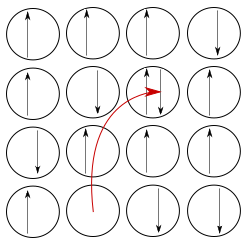
\includegraphics[width = 5cm]{hubbardOneHoleOneDoublyOc.png}
\caption{A configuration on the square lattice with a hole and a doubly occupied site.}
\end{figure}

If $a$ is large, we have essentially one electron per site at the start. When an electron is displaced, we end up with a hole and a doubly occupied site. The potential energy of such a state is

\begin{equation}
E_{H^-} + E_{H^+} - 2 E_H 
\end{equation}

Due to the Coulomb repulsion between the two electrons in $H^-$, this quantity is strictly positive. Call it $U > 0$. On the other hand, the system also has kinetic energy: both the hole and the doubly occupied site can delocalize. Let $W$ be the bandwidth corresponding to the delocalization of an electron on the lattice. Both the hole and the doubly occupied will stay at the bottom of the band and gain an energy $W/2$ (assuming that this delocalization is of the same order of magnitude). The dominant transfer integral $-t$ is between nearest neighbors. The dispersion relation then reads

\begin{equation}
\varepsilon_{\bm k} = -2 t ( \cos k_x + \cos k_y ) 
\end{equation}

The bandwidth is then $W = 8 t$. The energy of a configuration with a hole and a doubly occupied site is

\begin{equation}
\Delta_c = U - W ,
\end{equation}
where $U$ is practically independent of the lattice parameter $a$. The bandwidth $W$, however, depends strongly on $a$. When $a \gg a_0$, where $a_0$ is the Bohr radius, the transfer integral is exponentially small, because only the exponential tails of the wave functions are relevant. In this limit, $\Delta_c \approx U$ is a large, positive number, and the system is an insulator. This type of insulator is called a Mott insulator, and $\Delta_c$ is called the charge gap. As $a$ decreases, $t$ increases, and there must be a critical value $a_c \sim a_0$, for which $U = W$. Below this value, the computation of $\Delta_c$ is not valid anymore because the gap cannot be negative. Thus, there must be a metal-insulator transition. It is possible to see this transition if we apply enough pressure to a Mott insulator so as to decrease $a$ and increase $t$. A transition of this type was first seen in the 1970's for $V_2 O_3$\footnote{Of course, the transition is not so easy to describe. However, this simple argument provides an intuitive picture.}. There is a fundamental difference between a band insulator and a Mott insulator. While we must pay an energy $\Delta_c$ to make a charge excitation, this is not the cost of a spin excitation: we can flip the spin of an electron without creating a doubly occupied site. The fluctuations of both charge and spin due to the electron interactions may then lead to magnetic behavior characteristic of this type of systems.

\subsection{Effective Heisenberg Hamiltonian}\paragraph{}

Mott insulators allow low energy magnetic excitations (spin flips). The insulating phase corresponds to a configuration where each atom has an odd number of electrons, let's say one. This electron may have its spin up or down. In the purely atomic limit $\frac{t}{U} \rightarrow 0$, the atoms are infinitely far, and the excitation spectrum is very simple. The ground state is highly degenerate: every configuration with one electron per site is a ground state. As a matter of fact, the ground state is $2^N$-fold degenerate. The first excited state corresponds to configurations with a hole and a doubly occupied site. Let us set the energy of the ground state to zero in our conventions.  The energy of these configurations is then $U$, and there are $N(N-1)2^{N-2}$ of them. This process of generating higher energy excitations may be continued.

When the atoms are brought together, the first effect is the lifting of the degeneracy of the ground state, i.e. the splitting of the subspace of energy $E = 0$ in more subspaces. The effective hamiltonian describing the lifting of the degeneracy of the lowest energy band is obtained by applying degenerate perturbation theory \cite{Mila2007} to the kinetic term of the Hubbard Hamiltonian\footnote{An alternative method would be to use a canonical transformation technique.}

\begin{equation}
\mathcal{H}_0 = - t \sum_{\left\langle i, j \right\rangle, \sigma} ( c_{i\sigma}^\dagger c_{j\sigma} + c_{j\sigma}^\dagger c_{i\sigma} ) 
\end{equation}

\subsubsection{Two-site calculation}\paragraph{}

The effect of the hopping term is best understood in a minimal two-site example. There are four one-particle quantum states, represented by the action of the operators $c_{1,\uparrow}^\dagger$, $c_{1,\downarrow}^\dagger$, $c_{2,\uparrow}^\dagger$, $c_{2,\downarrow}^\dagger$ on the vacuum state. There are six two-particle states in the Fock space $\left| n_{1\uparrow} \,  n_{1\downarrow} \,  n_{2\uparrow} \, n_{2\downarrow} \right\rangle$:

\begin{equation}
\begin{split}
\left| 1 \right\rangle &\equiv \left| 1, 0, 1, 0 \right\rangle = c_{1\uparrow}^\dagger c_{2\uparrow}^\dagger \left| 0 \right\rangle \\
\left| 2 \right\rangle &\equiv \left| 0, 1, 0, 1 \right\rangle = c_{1\downarrow}^\dagger c_{2\downarrow}^\dagger \left| 0 \right\rangle \\
\left| 3 \right\rangle &\equiv \left| 1, 0, 0, 1 \right\rangle = c_{1\uparrow}^\dagger c_{2\downarrow}^\dagger \left| 0 \right\rangle \\
\left| 4 \right\rangle &\equiv \left| 0, 1, 1, 0 \right\rangle = c_{1\downarrow}^\dagger c_{2\uparrow}^\dagger \left| 0 \right\rangle \\
\left| 5 \right\rangle &\equiv \left| 1, 1, 0, 0 \right\rangle = c_{1\uparrow}^\dagger c_{1\downarrow}^\dagger \left| 0 \right\rangle \\
\left| 6 \right\rangle &\equiv \left| 0, 0, 1, 1 \right\rangle = c_{2\uparrow}^\dagger c_{2\downarrow}^\dagger \left| 0 \right\rangle \\
\end{split}
\end{equation}

The two-site Hamiltonian

\begin{equation}
\begin{split}
\mathcal{H}_{2} &= - t \bigg( c_{1\uparrow}^\dagger c_{2\uparrow} +  c_{2\uparrow}^\dagger c_{1\uparrow} + c_{1\downarrow}^\dagger c_{2\downarrow} +  c_{2\downarrow}^\dagger c_{1\downarrow} \bigg) \\
& + U (n_{1\uparrow}n_{1\downarrow} + n_{2\uparrow}n_{2\downarrow} )
\end{split}
\end{equation}
acts on the states of the Fock space as follows

\begin{equation}
\begin{split}
\mathcal{H}_{2}\left| 1 \right\rangle & = 0 \\
\mathcal{H}_{2}\left| 2 \right\rangle & = 0 \\
\mathcal{H}_{2}\left| 3 \right\rangle & =-t \big(c_{2\uparrow}^\dagger c_{1\uparrow} + c_{1\downarrow}^\dagger c_{2\downarrow} \big)c_{1\uparrow}^\dagger  c_{2\downarrow}^\dagger \left| 0 \right\rangle = -t \big( \left| 5 \right\rangle + \left| 6 \right\rangle \big)  \\
\mathcal{H}_{2}\left| 4 \right\rangle &=-t \big(c_{1\uparrow}^\dagger c_{2\uparrow} + c_{2\downarrow}^\dagger c_{1\downarrow} \big)c_{1\downarrow}^\dagger c_{2\uparrow}^\dagger \left| 0 \right\rangle = t \big( \left| 5 \right\rangle + \left| 6 \right\rangle \big) \\
\mathcal{H}_{2}\left| 5 \right\rangle & =\bigg[ -t \big(c_{2\uparrow}^\dagger c_{1\uparrow} + c_{2\downarrow}^\dagger c_{1\downarrow} \big) + U n_{1\uparrow}n_{1\downarrow}  \bigg]c_{1\uparrow}^\dagger c_{1\downarrow}^\dagger \left| 0 \right\rangle \\
&= U \left| 5 \right\rangle - t ( \left| 3 \right\rangle - \left| 4 \right\rangle )  \\
\mathcal{H}_{2}\left| 6 \right\rangle & = \bigg[ -t \big(c_{1\uparrow}^\dagger c_{2\uparrow} + c_{1\downarrow}^\dagger c_{2\downarrow} \big) + U n_{2\uparrow}n_{2\downarrow}  \bigg]c_{2\uparrow}^\dagger c_{2\downarrow}^\dagger \left| 0 \right\rangle \\
&= U \left| 6 \right\rangle - t ( \left| 3 \right\rangle - \left| 4 \right\rangle ) 
\end{split}
\end{equation}

When we act on the first two states we obtain $0$ because every term of the Hamiltonian gives a term $(c^\dagger)^2$, which is $0$ due to Pauli's exclusion principle. The minus signs that appear on the hopping terms stem from the fermion anticommutation relations.

Let us now diagonalize the Hamiltonian the subspace spanned by $\{\left| 3 \right\rangle, \left| 4 \right\rangle, \left| 5 \right\rangle, \left| 6 \right\rangle \}$. If we add states $\left| 3 \right\rangle$ and $\left| 4 \right\rangle $, we get $0$ when acting with the Hamiltonian. 

\begin{equation}
\mathcal{H}_{2} ( \left| 3 \right\rangle + \left| 4 \right\rangle ) = 0
\end{equation}

On the other hand, if we subtract $\left| 5 \right\rangle$ and $\left| 6 \right\rangle$, we obtain

\begin{equation}
\mathcal{H}_{2}(\left| 5 \right\rangle -\left| 6 \right\rangle) = U( \left| 5 \right\rangle - \left| 6 \right\rangle)
\end{equation}

We have found two more eigenvalues (the first two were trivially found to be zero). The others are found by subtracting $\left| 3 \right\rangle$ and $\left| 4 \right\rangle $ and adding $\left| 5 \right\rangle$ and $\left| 6 \right\rangle$.

\begin{equation}
\begin{split}
\mathcal{H}_{2} ( \left| 3 \right\rangle + \left| 4 \right\rangle ) &= -2 t  (\left| 5 \right\rangle + \left| 6 \right\rangle) \\
\mathcal{H}_{2}(\left| 5 \right\rangle -\left| 6 \right\rangle) &= - 2 t (\left| 3 \right\rangle - \left| 4 \right\rangle ) + U (\left| 5 \right\rangle + \left| 6 \right\rangle) 
\end{split}
\end{equation}

The characteristic equation allowing us to find the rest of the eigenvalues in the rotated subspace spanned by $\{\left| 3 \right\rangle \pm \left| 4 \right\rangle, \left| 5 \right\rangle \pm \left| 6 \right\rangle  \}$ is

\begin{equation}
\begin{split}
&E ( E - U ) - 4 t^2 = 0 \\
\iff&E_{\pm} = \frac{U \pm \sqrt{U^2 + 16 t^2}}{2}
\end{split}
\end{equation}

Taylor expanding the square root up to second order, we obtain

\begin{equation}
E_- = -\frac{4t^2}{U} \quad E_+ = U + \frac{4t^2}{U}
\end{equation}

Thus, we have obtained the complete energy spectrum. The ground state is a non-degenerate state of energy $-\frac{4t^2}{U}$, while the first excited state is a 3-fold degenerate state with energy $0$. The two other excited states have energies of the order of $U$, the first one being exactly $U$ and the second $U + \frac{4t^2}{U}$.

There are four sites for which the energy would be 0 if the hopping term vanished, corresponding to the four sites with one electron per site. The effect of the hopping term is to lift the degeneracy by splitting the 4-fold degenerate zero energy state into a singlet of energy $-\frac{4t^2}{U}$ and a triplet of energy $0$. This is what we obtain my minimizing a Heisenberg Hamiltonian of the form

\begin{equation}
\mathcal{H} = \frac{4t^2}{U} \bigg( \bm S_1 \cdot \bm S_2 - \frac{1}{4} \bigg)
\end{equation}
for two spins-$\frac{1}{2}$.

It turns out that this result is yet more general. For an arbitrary number of sites, this is is the form of the effective Hamiltonian at second order.

\subsubsection{Degenerate perturbation theory}\paragraph{}

To first order in $\mathcal{H}$, the matrix elements of its effective Hamiltonian coincide in the ground state subspace (by definition).

\begin{equation}
\left\langle m | \mathcal{H}_{\text{eff}} | n \right\rangle = \left\langle m | \mathcal{H}_0 | n \right\rangle ,
\end{equation}
where $| m \rangle$, and $| n \rangle$ belong to the ground state subspace. Since we are considering the system to be at half filling in our calculations, $| m\rangle$, and $| n \rangle$ must have one electron per site. The hopping Hamiltonian $\mathcal{H}_0$ makes an electron hop, leaving its previous site empty, and the site it hops to doubly occupied. This implies that all the matrix elements in the previous equation must be 0.

To second order, the matrix elements of the effective Hamiltonian are

\begin{equation}
\begin{split}
\left \langle m | \mathcal{H}_{\text{eff}} | n \right\rangle &= \sum_{ | k \rangle} \frac{\left\langle m | \mathcal{H}_0 | k \right\rangle \left\langle k | \mathcal{H}_0 | n \right\rangle }{E_0 - E_k} \\
&=-\frac{1}{U} \sum_{ | k \rangle} \left\langle m | \mathcal{H}_0 | k \right\rangle \left\langle k | \mathcal{H}_0 | n \right\rangle ,
\end{split}
\end{equation}
where $| k \rangle$ are the states that are not in the ground state subspace. In the second equality we simply noted that $\mathcal{H}_0$ creates a doubly occupied site. The energy cost of creating a doubly occupied site is $U$. 

The identity operator in the in the subspace of states with one doubly occupied site

\begin{equation*}
\sum_{ | k \rangle} | k \rangle \langle k |
\end{equation*}
may be written in a more convenient form in another representation:

\begin{equation*}
\sum_j n_{j,\sigma} n_{j, -\sigma}
\end{equation*}
so that the effective Hamiltonian becomes

\begin{equation}
\mathcal{H}_{\text{eff}} = - \mathcal{H}_0 \frac{\sum_j n_{j,\sigma} n_{j, -\sigma}}{U} \mathcal{H}_0
\end{equation}

For each element $j$ of the sum, only terms of type 

\begin{equation*}
\sum_{i(j)} c_{j\sigma}^\dagger c_{i\sigma} 
\end{equation*}
contribute. Here $\sum_{i(j)}$ is a sum over the set of neighbors $i$ of site $j$.

A term of the effective Hamiltonian $\mathcal{H}_{\text{eff}}$ corresponding to the j-th element in the sum reads

\begin{equation*}
-\frac{t^2}{U} \sum_{i(j), \sigma_1, \sigma_2 } c_{i,\sigma_1}^\dagger c_{j,\sigma_1} n_{j,\sigma} n_{j, -\sigma} c_{j, \sigma_2}^\dagger c_{i, \sigma_2}
\end{equation*}

There are only four cases in which the contribution of a term of this type is nonzero.

\begin{itemize}

\item $\sigma = \sigma_1 = \sigma_2$

The operator in the sum then becomes

\begin{equation*}
c_{i,\sigma}^\dagger c_{j,\sigma} n_{j,\sigma} n_{j, -\sigma} c_{j, \sigma}^\dagger c_{i, \sigma} = n_{i,\sigma} n_{j, -\sigma} c_{j,\sigma} n_{j, \sigma} c_{j, \sigma}^\dagger
\end{equation*}

Now, we use a fermionic operator identity:

\begin{equation*}
\begin{split}
&c n = c c^\dagger c = ( 1 -  c^\dagger c ) c = c \\
&\implies c_{j,\sigma} n_{j,\sigma} c_{j,\sigma}^\dagger = c_{j,\sigma} c_{j,\sigma}^\dagger = 1 - n_{j,\sigma}
\end{split}
\end{equation*}

The term of the Hamiltonian corresponding to this first case then takes on the form

\begin{equation*}
n_{i,\sigma} n_{j,-\sigma} ( 1 - n_{j, \sigma} )
\end{equation*}

We can further simplify this term by noting that in the subspace where $\mathcal{H}_{\text{eff}}$ acts, every site is occupied by only a single electron so that

\begin{equation*}
n_{j,\sigma} + n_{j,-\sigma} = 1 \iff 1 - n_{j,\sigma} = n_{j,-\sigma}
\end{equation*}

Since, for fermions we have that $\hat{n} = \hat{n}^k$, whichever the power $k \in \mathbbm{N}$, the final form of the sought term of the Hamiltonian is

\begin{equation*}
n_{i,\sigma} n_{j, -\sigma}
\end{equation*}

\item $-\sigma = \sigma_1 = \sigma_2$

The contribution to the Hamiltonian is exactly of the same form but making $\sigma \mapsto -\sigma$:

\begin{equation*}
n_{i,-\sigma} n_{j, \sigma}
\end{equation*}

\item $\sigma = - \sigma_1 = \sigma_2$

We can use the same reasoning as we did for the first term to obtain

\begin{equation*}
\begin{split}
&c_{i,-\sigma}^\dagger c_{j,-\sigma} n_{j,\sigma} n_{j, -\sigma} c_{j, \sigma}^\dagger c_{i, \sigma} \\
=& c_{i, -\sigma}^\dagger c_{i,\sigma} \underbrace{c_{j,-\sigma} n_{j, -\sigma}}_{c_{j,-\sigma}} \underbrace{n_{j, \sigma} c_{j, \sigma}^\dagger}_{c_{j,\sigma}^\dagger} \\
=& - c_{i, -\sigma}^\dagger c_{i,\sigma} c_{j, \sigma}^\dagger c_{j,-\sigma}
\end{split}
\end{equation*}

\item $-\sigma = - \sigma_1 = \sigma_2$

Analogously, the contribution to the Hamiltonian is

\begin{equation*}
\begin{split}
&c_{i,\sigma}^\dagger c_{j,\sigma} n_{j,\sigma} n_{j, -\sigma} c_{j, -\sigma}^\dagger c_{i, -\sigma} \\
=& - c_{i, -\sigma}^\dagger c_{i,\sigma} c_{j, \sigma}^\dagger c_{j,-\sigma}
\end{split}
\end{equation*}

\end{itemize}

Grouping all these four terms, we obtain

\begin{equation}
\mathcal{H}_{\text{eff}} = \frac{2t^2}{U} \sum_{\left\langle i, j \right\rangle, \sigma} ( - n_{i,\sigma} n_{j,-\sigma} + c_{i,-\sigma}^\dagger c_{i,\sigma} c_{j,\sigma}^\dagger c_{j,-\sigma} ) ,
\end{equation}
where the factor of 2 appears because for each pair of nearest neighbors $\left\langle i, j \right\rangle$, a term comes from the term $n_{j,\sigma} n_{j,-\sigma}$ of the sum $\sum_j n_{j,\sigma} n_{j,-\sigma}$, and another term from $n_{i,\sigma} n_{i,-\sigma}$.

Recall the second quantized form of the spin operators:

\begin{equation}
\begin{cases}
S_i^z = \frac{1}{2} ( n_{i,\uparrow} - n_{i,\downarrow} ) \\
S_i^+ = c_{i,\uparrow}^\dagger c_{i,\downarrow} \\
S_i^- = c_{i,\downarrow}^\dagger c_{i,\uparrow}, \\
\end{cases}
\end{equation}

Using these relations and that the density operator is $n_i = n_{i,\uparrow} + n_{i,\downarrow}$, the following relations hold

\begin{equation}
\begin{split}
S_i^z S_j^z - \frac{1}{4} n_i n_j &= -\frac{1}{2} ( n_{i,\uparrow} n_{j,\downarrow} + n_{i,\downarrow} n_{j,\uparrow} ) \\
S_i^+ S_j^- + S_i^- S_j^+ &= c_{i,\uparrow}^\dagger c_{i,\downarrow} c_{j,\downarrow}^\dagger  c_{j,\uparrow} +  c_{i,\downarrow}^\dagger c_{i,\uparrow} c_{j,\uparrow}^\dagger  c_{j,\downarrow}
\end{split}
\end{equation}

Thus, we may rewrite the effective Hamiltonian:

\begin{equation}
\mathcal{H}_{\text{eff}} = \frac{4t^2}{U} \sum_{\left\langle i, j \right\rangle} \bigg( S_i^z S_j^z - \frac{1}{4} n_i n_j + \frac{1}{2} ( S_i^+ S_j^- + S_i^- S_j^+ ) \bigg)
\end{equation}

But $S_i^z S_j^z + \frac{1}{2} ( S_i^+ S_j^- + S_i^- S_j^+) = \bm S_i \cdot \bm S_j$ and $n_i = n_j = 1$ in the ground state subspace, so the effective Hamiltonian becomes

\begin{equation}
\mathcal{H}_{\text{eff}} = \frac{4t^2}{U} \sum_{\left\langle i, j \right\rangle} \bigg( \bm S_i \cdot \bm S_j  - \frac{1}{4}  \bigg),
\end{equation}
which corresponds to the antiferromagnetic Heisenberg model: $\mathcal{H}_{\text{Heis}} = J \sum_{\left\langle i, j \right\rangle} \bm S_i \cdot \bm S_j $, with $J = 4 t^2 / U$. Since $J > 0$, the model favors configurations with antiparallel adjacent spins. There is an intuitive physical picture for this result: if two electrons on neighboring sites have parallel spins, none of the two can hop to the neighboring site due to Pauli's exclusion principle. If adjacent spins have antiparallel spins, however, it is possible for any of the two electrons to hop to the neighboring site, and this process allows the system to lower its energy.

As a final remark, we note that the effective Hamiltonian we obtained corresponds to the $\frac{t}{U} \ll 1$ limit, which is consistent since the Heisenberg model couples spins on different sites, thus it is an \emph{atomic} model.

\subsection{Exact solutions for simple cases}\label{exactSolutions}\paragraph{}

If we relax the condition of fixed number of particles, there is an extra energy term $-\mu N_p$ in the Hamiltonian (compared to equation (\ref{eq:hubbard_hamiltonian})), where $\mu$ is the chemical potential, and $N_p$ is the total number of particles. The Hubbard Hamiltonian may then be written as a sum of kinetic, chemical and potential energy terms, respectively:

\begin{equation}\label{eq:hubbard}
\mathcal{H} = \mathcal{H}_K + \mathcal{H}_\mu + \mathcal{H}_V ,
\end{equation}
defined as

\begin{equation}\label{eq:def_energies}
\begin{split}
\mathcal{H}_K &= -t \sum_{\left\langle i, j \right \rangle, \sigma} ( c_{i,\sigma} c_{j,\sigma}^\dagger + c_{j,\sigma}^\dagger c_{i,\sigma} ) \\
\mathcal{H}_\mu &= -\mu \sum_i ( n_{i,\uparrow} + n_{i,\downarrow} ) \\
\mathcal{H}_V &= U \sum_{i} ( n_{i,\uparrow} - \frac{1}{2} ) ( n_{i,\downarrow} - \frac{1}{2} )
\end{split} ,
\end{equation}
where:

\begin{itemize}
\item $i$ and $j$ label sites on the lattice.
\item $c_{i,\sigma}^{(\dagger)}$ is an operator that annihilates (creates) an electron with spin $\sigma$ on site $i$.
\item $n_{i,\sigma}$ is the number operator counting the number of electrons of spin $\sigma$ on site $i$ (either 0 or 1).
\item $t$ is the hopping parameter related to the kinetic energy of the electrons. It is determined by the overlap of the atomic wave functions on neighboring sites $\left\langle i, j \right\rangle$.
\item $U$ is the repulsive Coulomb interaction between electrons on the same lattice site. Whenever a site $i$ has two electrons, there is a local repulsion between them corresponding to an energy cost $U n_{i \uparrow} n_{i \downarrow}$. The constant $1/2$ terms serve to recast the Hamiltonian in particle-hole symmetric form.
\item $\mu$ is the chemical potential controlling the electron number (or density).
\end{itemize}

A given physical observable of interest $\mathcal{O}$, such as the spin-spin correlation, or the magnetic susceptibility may be computed formally by

\begin{equation}
\left\langle \mathcal{O} \right\rangle = \text{Tr} ( \mathcal{O} \mathcal{P} )
\end{equation}
where

\begin{equation}\label{eq:projection}
\mathcal{P} \equiv \frac{1}{Z} e^{-\beta \mathcal{H} } , \text{ with } Z = \text{Tr} ( e^{-\beta \mathcal{H} } )
\end{equation}

The trace is taken over the Hilbert space corresponding to all possible configurations of the lattice occupation. Defining an orthonormal basis of this Hilbert space $\{ | \psi_i \rangle | i = 1, ... D \} $, where $D$ is the dimension of the Hilbert space, the partition function reads

\begin{equation}\label{eq:z_asEigen}
\text{Tr} ( e^{-\beta \mathcal{H} } )= \sum_i \left\langle \psi_i | e^{-\beta \mathcal{H} } | \psi_i \right\rangle
\end{equation}

There are four possible states at each site in the Hubbard model: $\left| \,\, \right\rangle$, $\left|\uparrow \right\rangle$, $\left|\downarrow\right \rangle$, $\left|\uparrow \downarrow \right\rangle $, corresponding, respectively, to no electron, spin up or spin down electron, and two electrons occupying the site. The potential energy operator acts as follows

\begin{equation}
U (n_{i\uparrow} - \frac{1}{2} ) ( n_{i\downarrow} - \frac{1}{2} ) 
\begin{cases}
\left| \,\, \right\rangle = \frac{U}{4} \left| \,\, \right\rangle \\
\left|\uparrow \right\rangle = -\frac{U}{4} \left|\uparrow \right\rangle \\
\left|\downarrow\right \rangle = -\frac{U}{4} \left|\downarrow\right \rangle \\
\left|\uparrow \downarrow \right\rangle = \frac{U}{4} \left|\uparrow \downarrow \right\rangle \\
\end{cases}
\end{equation}

Singly occupied states ($\left|\uparrow \right\rangle$, $\left|\downarrow\right \rangle$) have lower energy and are thus more likely to occur. They correspond to nonzero magnetization $m = n_{\uparrow} - n_{\downarrow}$, which is favored by the Hubbard interaction $U$. A relevant question is whether or not the spins order in space when $t \neq 0$.

Let us now establish our notations for second quantized operators to introduce a different representation of electronic states on the lattice. The fermionic annihilation and creation operators anticommute.

\begin{equation}
\{ c_{j\sigma} , c_{l \sigma'}^\dagger \} = \delta_{jl} \delta_{\sigma\sigma'}
\end{equation}

The $c$-operator algebra is further defined by the vanishing of all other anticommutators.

\begin{equation}\label{eq:fermion_anticom}
\{ c_{j\sigma}^{(\dagger)} , c_{l \sigma'}^{(\dagger)} \} = 0
\end{equation}

Note that taking $l = j$ and $\sigma = \sigma'$ in equation (\ref{eq:fermion_anticom}), we recover Pauli's exclusion principle since $(c_{j\sigma}^\dagger)^2 = 0$. If we omit the site index $i$ and spin $\sigma$, a convenient way of specifying states on the lattice is

\begin{equation}
\begin{split}
&\left| 0 \right\rangle : \text{unoccupied state - no electron} \\
&\left| 1 \right\rangle : \text{occupied state - one electron}
\end{split}
\end{equation}
so that a generic state may be written as a product of the states above $\otimes_{i=1}^{N} \otimes_{\sigma = \pm 1/2} \left| n \right\rangle_{i, \sigma}$ at each site for each spin state, where $n= 0, 1$. For example, one such state is

\begin{equation}
\left| 0 \right\rangle_{1, 1/2} \left| 1 \right\rangle_{1, -1/2} \left| 0 \right\rangle_{2, 1/2} \left| 0 \right\rangle_{2, -1/2} ... \left| 0 \right\rangle_{N, 1/2} \left| 1 \right\rangle_{N, -1/2}  ,
\end{equation}
where $N$ is the number of sites on the lattice.

The creation and annihilation operators act as follows

\begin{equation}
c \left| 0 \right\rangle = 0 \quad c^\dagger \left| 0 \right\rangle = \left| 1 \right\rangle \quad c \left| 1 \right\rangle = \left| 0 \right\rangle \quad c^\dagger \left| 1 \right\rangle = 0
\end{equation}

Thus, the eigenstates of the number operator are $\left| 0 \right\rangle, \left| 1 \right\rangle$:

\begin{equation}
n \left| 0 \right\rangle = 0 \quad n \left| 1 \right\rangle = \left| 1 \right\rangle
\end{equation}

Moreover, the operator $c_i^\dagger c_{i+1}^\dagger$, corresponding to the hopping from site $i+1$ to $i$, i.e. to the kinetic energy of the electrons on neighboring sites, acts as follows (ignoring spin):

\begin{equation}
c_i^\dagger c_{i+1}^\dagger \begin{cases}
\left|0 0 \right\rangle = 0 \\
\left|1 0 \right\rangle =  0 \\
\left|0 1 \right\rangle =  \left| 1 0 \right\rangle \\
\left|1 1 \right\rangle =  c_i^\dagger \left| 1 0  \right\rangle = 0 \\
\end{cases}
\end{equation}

The operator annihilates the particle at $i+1$ and creates it back at $i$, i.e. the electron hops from $i+1$ to $i$.

\subsection{The purely atomic $\frac{t}{U} = 0$ limit}\paragraph{}

When $t = 0$, the Hamiltonian reduces to 

\begin{equation}
\mathcal{H} = U (n_\uparrow - \frac{1}{2} ) (n_\downarrow - \frac{1}{2} ) - \mu ( n_\uparrow + n_\downarrow )
\end{equation}
which acts as follows (using the eigenstates of $n_\sigma$)

\begin{equation}
\mathcal{H} \begin{cases}
\left| \,\, \right\rangle = \frac{U}{4} \\
\left| \uparrow \right\rangle = \bigg( \frac{U}{4} - (\mu + \frac{U}{2} ) \bigg) \left| \uparrow \right\rangle \\
\left| \downarrow \right\rangle = \bigg( \frac{U}{4} - (\mu + \frac{U}{2} ) \bigg) \left| \downarrow \right\rangle \\
\left| \uparrow \downarrow \right\rangle = \bigg( \frac{U}{4} - 2 \mu \bigg) \left| \uparrow \downarrow \right\rangle
\end{cases}
\end{equation}

Thus, the Hamiltonian is diagonal in the basis $\{\left| \psi_i \right\rangle \}$:

\begin{equation}
\begin{split}
&\bigg[ \mathcal{H}_{ij} \bigg] = \bigg[ \left\langle \psi_i \left| \mathcal{H} \right| \psi_j \right\rangle \bigg] \\
&= \text{diag}\bigg(\frac{U}{4}, \frac{U}{4} - (\mu + \frac{U}{2} ), \frac{U}{4} - (\mu + \frac{U}{2} ), \frac{U}{4} - 2 \mu \bigg) ,
\end{split}
\end{equation}
which means that $e^{-\beta \mathcal{H} }$ is also diagonal:

\begin{equation}
e^{-\beta \mathcal{H} } = e^{-\beta U / 4}  \text{diag}\bigg(1,  e^{\beta(\mu + \frac{U}{2})}, e^{\beta(\mu + \frac{U}{2})},  e^{2\beta \mu} \bigg)
\end{equation}
and this is one of the rare situations in which it is possible to explicitly write down a closed form for the partition function.

\begin{equation}
\begin{split}
Z &= \text{Tr} ( e^{-\beta\mathcal{H} } ) = \sum_i \left\langle \psi_i \left|e^{-\beta \mathcal{H} } \right| \psi_i \right\rangle \\
&= e^{-\beta U / 4} \bigg(1 + 2 e^{\beta(\mu + \frac{U}{2})} + e^{2 \beta \mu} \bigg)
\end{split}
\end{equation}

Moreover, some of the observables that were mentioned before are explicitly computable. This is because due to the diagonal form of $\mathcal{H}$, the expressions defining these observables greatly simplify.

\begin{equation}
\begin{split}
\mathcal{H} e^{-\beta\mathcal{H} } &\mapsto e^{-\beta U / 4}  \text{diag}\bigg(\frac{U}{4}, (-\mu - \frac{U}{4})  e^{\beta(\mu + \frac{U}{2})}, \\ 
&(-\mu - \frac{U}{4}) e^{\beta(\mu + \frac{U}{2})}, (\frac{U}{4} - 2\mu ) e^{2\beta \mu} \bigg) \\
n_{\uparrow} e^{-\beta\mathcal{H} } &\mapsto e^{-\beta U / 4}  \text{diag}\bigg(0, e^{\beta(\mu + \frac{U}{2})}, 0,  e^{2\beta \mu} \bigg) \\
n_{\downarrow} e^{-\beta\mathcal{H} } &\mapsto e^{-\beta U / 4}  \text{diag}\bigg(0, 0, e^{\beta(\mu + \frac{U}{2})},   e^{2\beta \mu} \bigg) \\
n_{\uparrow} n_{\downarrow} e^{-\beta\mathcal{H} } &\mapsto e^{-\beta U / 4}  \text{diag}\bigg(0, 0, 0,   e^{2\beta \mu} \bigg) \\
\end{split}
\end{equation}

From these we can compute some useful traces

\begin{equation}
\begin{split}
&\text{Tr} \bigg( \mathcal{H} e^{-\beta\mathcal{H} } \bigg) = e^{-\beta U / 4} \bigg(\frac{U}{4} + 2 (-\mu - \frac{U}{4})  e^{\beta(\mu + \frac{U}{2})} \\
& + (\frac{U}{4} - 2\mu ) e^{2\beta \mu} \bigg) \\
&\text{Tr} \bigg( (n_\uparrow + n_\downarrow ) e^{-\beta\mathcal{H} } \bigg) = e^{-\beta U / 4} \bigg(2 (-\mu - \frac{U}{4})  e^{\beta(\mu + \frac{U}{2})} \\
& + (\frac{U}{4} - 2\mu ) e^{2\beta \mu} \bigg) \\
&\text{Tr} \bigg( n_\uparrow n_\downarrow \bigg) = e^{-\beta U/4} e^{2\beta\mu}
\end{split}
\end{equation}

The bottom line is that we are able to obtain \emph{exact} expressions for

\begin{enumerate}
\item the one-site density $\rho = \left\langle n_\uparrow \right\rangle + \left\langle n_\downarrow \right\rangle$, measuring the average occupation of each site.
\begin{equation}
\begin{split}
\rho &= \frac{\text{Tr} \big[ (n_\uparrow + n_\downarrow ) e^{-\beta\mathcal{H}} \big]}{Z} \\
&= \frac{2 e^{\beta(\frac{U}{2} + \mu)} + 2 e^{2\beta\mu}}{1 + 2 e^{\beta(\mu + \frac{U}{2})} + e^{2 \beta \mu}}
\end{split}
\end{equation}

Note that when there is no chemical potential $\mu = 0$, we have $\rho = 1$ for any $U$, or $\beta$. This corresponds to half filling: the density of electrons is half its maximum possible value.

\item the one-site energy $E = \left\langle \mathcal{H} \right\rangle$.
\begin{equation}
\begin{split}
E &= \frac{\text{Tr}\bigg( \mathcal{H}e^{-\beta\mathcal{H} } \bigg)}{Z} \\
&= \frac{ \frac{U}{4} + 2 ( -\mu - \frac{U}{4} ) e^{\beta(\frac{U}{2} + \mu )} + (\frac{U}{4} - 2\mu ) e^{2\beta\mu}}{1 + 2 e^{\beta (\frac{U}{2} + \mu )} + e^{2\beta\mu} } \\
&= \frac{ \frac{U}{4} ( 1 + 2 e^{\beta (\frac{U}{2} + \mu )} + e^{2\beta\mu} )}{1 + 2 e^{\beta (\frac{U}{2} + \mu )} + e^{2\beta\mu} } \\
&+ \frac{2(-\mu - \frac{U}{4}) e^{\beta(\frac{U}{2} + \mu)} - 2\mu e^{2\beta\mu} - 2\frac{U}{4} e^{\beta (\frac{U}{2} + \mu)} }{1 + 2 e^{\beta (\frac{U}{2} + \mu )} + e^{2\beta\mu}} \\
&= \frac{U}{4} - \frac{ (2\mu - U) e^{\beta(\frac{U}{2} + \mu) } + 2\mu e^{2\beta\mu} }{1 + 2 e^{\beta (\frac{U}{2} + \mu )} + e^{2\beta\mu} }
\end{split}
\end{equation}
which at half filling becomes

\begin{equation}
E = \frac{U}{4} - \frac{U}{2 ( 1 + e^{-\beta U /2} )}
\end{equation}

\item the double occupancy $\left\langle n_\uparrow n_\downarrow \right\rangle$.

\begin{equation}
\left\langle n_\uparrow n_\downarrow \right\rangle = \frac{\text{Tr} \big[ n_\uparrow n_\downarrow \big]}{Z} = \frac{e^{2\beta\mu}}{1 + 2 e^{\beta (\frac{U}{2} + \mu )} + e^{2\beta\mu}}
\end{equation}
which, at half filling, simplifies to

\begin{equation}
\left\langle n_\uparrow n_\downarrow \right\rangle = \frac{1}{2 ( 1 + e^{\beta U/2} )}
\end{equation}

Note that as either $U$ or $\beta$ increase the double occupancy tends to zero.
\end{enumerate}

\subsection{The non-interacting $\frac{t}{U} \rightarrow \infty$ limit}\paragraph{}

In the $\frac{t}{U} \rightarrow \infty$ limit, the spin spaces become independent, and they may be considered separately. Thus we omit the spin indices of the operators in the Hamiltonian:

\begin{equation}
\mathcal{H} = -t \sum_{\left\langle i j \right\rangle} \big( c_i^\dagger c_j + c_j^\dagger c_i \big) - \mu \sum_i n_i
\end{equation}
which may be recast as a bilinear form

\begin{equation}
\mathcal{H} = \bm c^\dagger ( -t \bm K - \mu \bm I ) \bm c ,
\end{equation}
where

\begin{equation}
\bm c = \bigg[ c_1 \,\, c_2 \,\, ... \,\, c_N \bigg]^T \quad \bm c^\dagger = \bigg[c_1^\dagger \,\, c_2^\dagger \,\, ... c_N^\dagger \bigg]
\end{equation}
and $\bm I$ is the identity matrix. We also defined a matrix of zeros and ones specifying the hopping geometry $\bm K$. When writing down $\bm K$, we must specify the boundary conditions. Periodic boundary conditions (PBC) preserve a system's translational invariance and are advantageous because they reduce finite size effects. An example of a quantity which is measured more accurately is energy. In the thermodynamic limit, $N \rightarrow \infty$, the measured energy differs from the actual value by a correction of order $\mathcal{O}(\frac{1}{N^2})$ with PBC, while for open boundary conditions (OBC), the correction is of order $\mathcal{O}(\frac{1}{N})$. PBC have the property of giving site independent observables. For example, the electron density per site does not vary with PBC, but it varies with the distance to the edges of the lattice when we use OBC.

Consider a rectangular two-dimensional lattice with $N_x \times N_y$ sites. Then, we have $\dim(\bm K) = N_x N_y \times N_x N_y $, and

\begin{equation}
\bm K = \bm I_y \otimes \bm K_x + \bm I_x \otimes \bm K_y ,
\end{equation}
where $\bm I_{x, y}$ are identity matrices of dimension $N_{x, y}$, respectively.

For lattices in 1D or 2D, it is possible to find an exact eigendecomposition

\begin{equation}
\bm K = \bm F^T \bm \Lambda \bm F \quad \text{with}  \quad \bm F^T \bm F = \bm I ,
\end{equation}
where $\bm \Lambda = \text{diag}(\lambda_k)_{k = 1}^{N_x N_y}$ is a diagonal matrix of eigenvalues of $\bm K$. The Hamiltonian is diagonalized:

\begin{equation}\label{eq:quadraticH}
\mathcal{H} =\tilde{\bm c}^\dagger \big( -t \bm K - \mu \bm I \big) \tilde{\bm c} = \sum_k \varepsilon_k \tilde{n}_k ,
\end{equation}
where $\tilde{\bm c} = \bm F \bm c$ and $\tilde{\bm c}^\dagger = (\bm F \bm c)^\dagger$, and

\begin{equation}
\varepsilon_k = -t \lambda_k - \mu \quad \tilde{n}_k = \tilde{c}_k^\dagger \tilde{c}_k
\end{equation}

The $\tilde{c}$-operators are equally valid electron creation/annihilation operators, obeying the same anticommutation relations as the original operators $c_i$. While the original operators create/annihilate particles at specific (spatial) sites, the new ones create/annihilate particles with momentum $k$. Both sets of operators describe the same physics, however the interaction term in the Hubbard model is fairly complex to write in momentum space so it is not possible to apply this procedure to diagonalize it.

\bigskip

Now, it turns out that it is easy to evaluate the partition function for quadratic Hamiltonians. If $\mathcal{H} = \bm c^\dagger \bm H \bm c$, where $\bm H$ is a $N \times N$ Hermitian matrix, then we have that

\begin{equation}\label{eq:trace_quadratic}
\text{Tr} \big[ e^{-\beta \mathcal{H} } \big] = \prod_{i=1}^N ( 1 + e^{-\beta \lambda_{k_i} } ) ,
\end{equation}
where $\lambda_{k_i}$ are the eigenvalues of $\bm H$.

\bigskip

Thus, we would like to devise some approximation to transform the quartic term of the Hubbard model in a quadratic form. This will come shortly. Let us first finish the solution of the non-interacting case. We proceed by proving equation (\ref{eq:trace_quadratic}). Without loss of generality, let us consider $\bm H$ to be diagonal. Then, its eigenvalues coincide with the diagonal entries, so that $\bm H = \text{diag}(\lambda_{k_i} )$. The quadratic Hamiltonian may then be  diagonalized

\begin{equation*}
\mathcal{H} = {\bm c}^\dagger \text{diag} (\lambda_{k_1}, \lambda_{k_2}, .., \lambda_{k_N}) \bm c = \sum_{i=1}^N \lambda_{k_i} n_{k_i}
\end{equation*}

We continue by induction. When $N=1$, we have

\begin{equation*}
\begin{split}
\text{Tr} (e^{-\beta\mathcal{H} } ) &= \left\langle 0 \left| e^{-\beta \lambda_{k_1} n_{k_1}}  \right| 0 \right\rangle + \left\langle 1 \left| e^{-\beta \lambda_{k_1} n_{k_1}}   \right| 1 \right\rangle \\
&= 1 + e^{-\beta \lambda_{k_1} }
\end{split}
\end{equation*}

Assuming that for $N-1$:

\begin{equation*}
\text{Tr} \big[ e^{-\beta \sum_{i=1}^{N-1} \lambda_{k_i} n_{k_i} } \big] = \prod_{i=1}^{N-1} ( 1 + e^{-\beta \lambda_{k_i} } )
\end{equation*}
we compute the trace for $i$ going up to $N$.

\begin{equation*}
\begin{split}
&\text{Tr} \big[ e^{-\beta \sum_{i=1}^{N-1} \lambda_{k_i} n_{k_i} } \big] = \\
& \sum_{\{ k_i \}_{i=1}^{N} } \left\langle \psi_1^{k_1} \psi_2^{k_2} ... \psi_N^{k_N} \left| e^{-\beta \sum_{i=1}^N \lambda_{k_i} n_{k_i}}  \right| \psi_1^{k_1} \psi_2^{k_2} ... \psi_N^{k_N} \right\rangle = \\
& \sum_{\{ k_i \}_{i=1}^{N-1} } \bigg( \left\langle \{\psi_i^{k_i}\} 0 \left| e^{-\beta \sum_{i=1}^N \lambda_{k_i} n_{k_i}} e^{-\beta \lambda_{k_N} n_{k_N}} \right| \{\psi_i^{k_i}\} 0 \right\rangle \\
&+ \left\langle \{\psi_i^{k_i}\} 1 \left| e^{-\beta \sum_{i=1}^N \lambda_{k_i} n_{k_i}} e^{-\beta \lambda_{k_N} n_{k_N}} \right| \{\psi_i^{k_i}\} 1 \right\rangle \bigg) \\
&= (1 + e^{-\beta \lambda_{k_N} } ) \sum_{\{ k_i \}_{i=1}^{N-1} } \left\langle \{\psi_i^{k_i}\} \left| e^{-\beta \lambda_{k_i} n_{k_i}} \right| \{\psi_i^{k_i}\} \right\rangle \\
&= (1 + e^{-\beta \lambda_{k_N} } ) \prod_{i=1}^{N-1} (1 + e^{-\beta \lambda_{k_i} } ) \\
&= \prod_{i=1}^{N} (1 + e^{-\beta \lambda_{k_i} } )
\end{split}
\end{equation*}

To complete the proof we note that for any $\bm H$, there exists a unitary matrix $\bm Q$, such that $\bm Q^T \bm H \bm Q = \bm \Lambda = \text{diag}(\lambda_{k_i})$. Let $\tilde{\bm c} = \bm Q \bm c$, and $\tilde{n_i} = \tilde{c_i}^\dagger \tilde{c_i}$. Then, we find

\begin{equation*}
\mathcal{H} = \bm c^\dagger \bm H \bm c = \bm \tilde{\bm c}^\dagger \bm \Lambda \tilde{\bm c} = \sum_{i=1}^N \lambda_{k_i} \tilde{n}_{k_i}
\end{equation*}

The trace is independent of the choice of basis functions. Thus, we have

\begin{equation*}
\begin{split}
\text{Tr} ( e^{-\beta \mathcal{H} } ) &= \text{Tr} \bigg( \prod_{i=1}^N e^{-\beta \lambda_{k_i} \tilde{n}_{k_i} } \bigg) \\
&= \prod_{i=1}^N \bigg( 1 + e^{-\beta \lambda_{k_i} } \bigg) \quad\quad \qedsymbol
\end{split}
\end{equation*}

This result may be applied to compute the partition corresponding to the quadratic Hamiltonian defined in equation (\ref{eq:quadraticH}).

\begin{equation}
Z = \prod_k ( 1 + e^{-\beta \varepsilon_k} )
\end{equation}
and it is again possible to find closed form expressions for observables of interest.

\begin{enumerate}
\item the density, or average occupation of each site, $\rho$.

\begin{equation}
\rho = \left\langle n \right\rangle = \left\langle \tilde{n} \right\rangle = \frac{1}{N} \sum_{k=1}^N \left\langle \tilde{n}_k \right\rangle  = \frac{1}{N} \sum_{k=1}^N  \frac{1}{1 + e^{\beta\varepsilon_k}}
\end{equation}

\item the energy $E = \left\langle \mathcal{H} \right\rangle$.

\begin{equation}
E = \frac{1}{N} \sum_k \frac{\varepsilon_k}{1 + e^{\beta\varepsilon_k}}
\end{equation}

\item the equal-time Green's function, which plays a key role in computing other quantities, such as correlation functions.

\begin{equation}
G_{lj} = \left\langle c_l c_j^\dagger \right\rangle = \frac{1}{N} \sum_k e^{ i k \cdot ( l - j ) } ( 1 - f_k ),
\end{equation}
where $f_k = \big(1 + e^{\beta(\varepsilon_k - \mu)} \big)^{-1}$ is the Fermi-Dirac distribution. Note that the Green function, like the Hamiltonian, is translationally invariant: $G_{lj} = G_{l-j}$. If we use PBC, no site is singled out, they are all equivalent and this behavior of the Green's function should become apparent.
\end{enumerate}

\section{Simulations}\label{hubbQMC}\paragraph{}

The Monte Carlo method is ubiquitous. Its central idea is to use randomness to produce accurate estimates of deterministic integrals. The term was coined by Nicolas Metropolis in 1949, first appearing in a seminal paper, in which it was described as a \say{statistical approach to the study of differential equations, or more generally, of integro-differential equations that occur in various branches of sciences}\cite{Metropolis1949}. Although it was used as early as 1777 in an experiment known as Buffon's needle - where one obtains an estimate of the constant $\pi$ by repeatedly throwing  a needle randomly onto a sheet of paper with evenly spaced lines - it was crucially developed in the Los Alamos National Laboratory during World War II where the development of the first atomic bomb was completed, the primary objective of the Manhattan Project. The method is particularly useful when one wants to sample from a probability distribution in an exponentially large state space. In fact, it can in principle be used to solve any problem allowing a probabilistic formulation.

\subsection{Classical vs Monte Carlo}\paragraph{}

The law of large numbers affords an approximation to integrals which can be written as an expectation of a random variable. Upon drawing enough independent samples from the corresponding distribution, the sample mean gets arbitrarily close to the integral at stake.

\begin{equation}\label{eq:int_mean}
\mathbb{E} [f(X)] = \int dx f(x) p(x),
\end{equation}
where $p(x)$ is the distribution of $X$. 

We could simply draw $M$ independent and identically distributed samples $x_{1,...M}$ from $p(x)$ and approximate the integral as

\begin{equation}
\frac{1}{M} \sum_{k=1}^M f (x_k) , 
\end{equation}
which in most cases converges to the desired expectation, as long as $M$ is large enough. How large?

\begin{equation}\label{eq:variance}
\text{Var}\bigg( \frac{1}{M} \sum_{k=1}^M f(x_k) \bigg) = \frac{1}{M} \text{Var}\bigg( f(x_1) \bigg) \sim \mathcal{O}\bigg(\frac{1}{M}\bigg)
\end{equation}

Thus, the correction to the sample mean is of order $\mathcal{O}(M^{-1/2})$.

How do we sample from an arbitrary distribution $p(X)$? The idea is to first make an educated choice of a Markov Chain with the prescribed stationary distribution from which we ultimately desire to sample from, $p(X)$. After a sufficiently high number of steps, a Markov Chain Monte Carlo (MCMC) algorithm generates samples from the target distribution. Imposing some conditions on this Markov Chain, namely that it should be irreducible, aperiodic and positive recurrent, the ergodic theorem guarantees that the empirical measures of the aforementioned sampler approach the target stationary distribution. Another important condition to impose on this Markov Chain is detailed balance. Let the transition matrix be $\bm P = [p_{ij}]$, and the state space $\Omega$ be $\{\pi_i | i=1, ..., |\Omega| \}$, where $|\Omega|$ is the total number of possible states. Then, the condition of detailed balance is defined for all $i, j$ as

\begin{equation}
\pi_i p_{ij} = p_{ji} \pi_j 
\end{equation}

Crucially, Monte Carlo methods employ \emph{importance sampling}. It turns out that we can improve upon our estimate of $\mathbb{E} [f(X)]$ by introducing a separate distribution $q(x)$, and defining the weight function as $w(x) = p(x)/ q(x)$. Then, we can rewrite equation (\ref{eq:int_mean}):

\begin{equation}
\mathbb{E} [f(X)] = \int dx f(x) q(x) w(x) = \mathbb{E} [f(Y) w(Y)],
\end{equation}
with $Y \sim q$, i.e. the random variable $Y$ follows the distribution $q(Y)$

It appears as though we didn't gain anything. However, by choosing $q$ wisely, we can actually reduce the variance we computed in equation (\ref{eq:variance}):

\begin{equation}
\text{Var}\bigg( \frac{1}{M} \sum_{k=1}^M f(y_k) w(y_k) \bigg) = \frac{1}{M} \text{Var}\bigg( f(y_1) w(y_1) \bigg)
\end{equation}

Since we didn't make any assumptions about $q(Y)$, it may be chosen so as to minimize the variance, hence the error of the Monte Carlo estimator, improving the approximation of the expectation. However, note that the error remains of order $\mathcal{O}\big(\frac{1}{\sqrt{M}}\big)$.

The idea of the Quantum (Classical) Monte Carlo method is to simulate the random quantum (thermal) fluctuations of the system, as it oscillates between states in a given time frame \cite{Newman1999}. Instead of visiting these states uniformly, the algorithm applies \emph{importance sampling}: the most relevant part of the phase space is sampled more frequently, overcoming the seemingly exponential complexity of computing a sample mean numerically. Even though only a small fraction of the system's states are sampled, we obtain an accurate estimate of physical quantities of interest, namely energy, and correlation functions.

QMC generally provides an accurate approximation of the solution to the quantum many-body problem. When relativistic effects are negligible, which is the case of most condensed matter systems, any physical system can be described by a many-body Schr\"odinger equation. The issue is that the many-body wave function lives in the corresponding Hilbert space that is  exponentially large in the number of particles. For example, the number of possible states of a physical system whose configuration space rests on a two-dimensional lattice is exponentially large. The method described above is applied to approximate the multidimensional integrals arising upon formulating the quantum many-body problem in this space.

One can set up a na\"ive mean field theory in which the many body wave function is approximated by an antisymmetric function of one body wave functions\footnote{This corresponds to the Hartree-Fock approximation that we used to derive the Hubbard Hamiltonian in section \ref{hubbardHamiltonian}.}. One of the drawbacks of this approach is that the effect of  correlations is not captured. Fermionic QMC goes beyond mean field theory,  capturing the phenomena occuring within strongly correlated electronic systems. For non-frustrated boson systems, a polynomially scaling algorithm leads to an exact solution. For a fermionic system, such as the TMD nanoribbon, the existing algorithms usually provide accurate yet not exact solutions, which would in general require exponential computing time. This is due to the so called sign problem. We will discuss this numerical issue later. 

\subsection{Variational Techniques}\paragraph{}

It is natural to combine a sampling scheme, such as the Metropolis algorithm, with a variational principle. The goal then becomes that of finding a variational many-fermion wave function which can be optimized so that ultimately we obtain as accurate as possible an estimate of the ground state of the system and then use it to evaluate averages of physical observables for zero temperature, $T=0$.

The parameters $[\alpha_i]$ of a trial wave function $\phi(\bm r)$ are optimized according to the variational principle

\begin{equation}
E[\alpha_i] = \frac{\left\langle \phi \left| \mathcal{H} \right| \phi \right\rangle}{\left\langle \phi | \phi \right\rangle} \ge E_0,
\end{equation}
where $E_0$ is the ground state energy.

In fact, expanding in terms of the eigenstates of the hamiltonian $\{ \psi_n (\bm r) \}$, a complete basis set:

\begin{equation}
\phi (\bm r) = \sum_{n= 0}^{\infty} a_n \psi_n (\bm r) ,
\end{equation}
and plugging it back into the variational principle, subject to $E_n \ge E_0 ,\, n > 0$ and $\left\langle \psi_n | \psi_m \right\rangle = \delta_{nm}$ we obtain

\begin{equation}
E[\alpha_i] = \frac{\sum_n a_n^2 E_n}{\sum_n a_n^2 } \ge E_0
\end{equation}

The expectation is the integral

\begin{equation}
E[\alpha_i] = \frac{\int \phi^\star (\bm r) \mathcal{H} \phi (\bm r) d\bm r}{\int | \phi (\bm r') |^2 d\bm r'} \equiv \int W(\bm r) E_L(\bm r) d\bm r ,
\end{equation}
where the integrand is a quantity which may be regarded as a distribution function 

\begin{equation}
W(\bm r) = \frac{|\phi (\bm r)|^2}{\int |\phi(\bm r')|^2 d\bm r'}
\end{equation}
multiplied by a local energy of the system at $\bm r$:

\begin{equation}
 E_L(\bm r) = \frac{\mathcal{H}\phi(\bm r)}{\phi (\bm r)}
\end{equation}

Given $W(\bm r)$ and $E_L(\bm r)$, one can in principle evaluate $E[\alpha_i]$. In practice, $\phi (\bm r) $ is parametrized depending on the physical model at play, and the variational parameters $\{\alpha_i\}$ in the trial wave function are optimized by minimizing $E[\alpha_i]$.\par

The Metropolis algorithm, for instance, may be used to sample a set of points $\{\bm r_k\}_{i=1}^M$, where $M$ is the number of Monte Carlo \say{measurements}, and the evaluation of the expectation value $E[\alpha_i]$ in each QMC step for each set of variational parameters is the equivalent of computing an average of a classical quantity at a given temperature in classical Monte Carlo. Systematically, we optimize the wave function based on the Euler-Lagrange equation

\begin{equation}
\frac{\delta E[\alpha_i]}{\delta \alpha_j} = 0
\end{equation}

\subsection{Diffusion Monte Carlo}\label{subsec:dmc}\paragraph{}

The variational approach is limited by the use of a trial wave function $\phi (\bm r)$: we may not have enough information to even construct a reliable variational wave function in the first place. 

Diffusion Quantum Monte Carlo (DQMC) allows the simulation of a many-body system even when having only a limited \emph{a priori} knowledge of the system's physical properties. The problem is that while it is exact for many-boson systems, it is only approximate for many-fermion systems. The idea is to map the Schr\"odinger equation onto  an imaginary-time diffusion equation. Excited states are then filtered out by a diffusion process as time passes. In imaginary-time $\tau =  i t$, the solution to Schr\"odinger's equation in terms of a formal series expansion in the eigenfunctions of the hamiltonian becomes a series of transients $e^{-E_n \tau}, \, n \in \mathbb{N}$. The longest lasting of these is the ground state. \cite{Kosztin1996} \par

The idea of DQMC is to generate samples using the exact ground state wave function $\phi_0 (\bm r)$ \cite{Toulouse2016, Pang2016}. The associated exact energy $E_0$ is the matrix element of the hamiltonian calculated using a trial wave function and the ground state wave function.

\begin{equation}
\begin{split}
&E_0 = \frac{ \left\langle \phi_0 | E_0 | \phi \right\rangle}{\left\langle \phi_0 | \phi \right\rangle} = \\
&= \frac{\left\langle \phi_0 | \mathcal{H} | \phi \right\rangle}{ \left\langle\phi_0 | \phi \right\rangle} = \frac{\int d\bm r \phi_0^\star (\bm r) \phi (\bm r) E_L (\bm r)}{\int d\bm r\phi_0^\star (\bm r) \phi (\bm r)}
\end{split}
\end{equation}

Note that using this trick we avoid the computation of $\mathcal{H} \phi_0 = E_0 \phi_0$, that is, the ground state energy. Instead, we approximate the integral by considering $M$ configuration samples $\bm r_{k = 1,..., M}$ in a similar spirit to that of variational QMC. Notice that the integral consists of a local energy of the trial wave function $E_L (\bm r) = \frac{\mathcal{H} \phi (\bm r)}{\phi (\bm r)}$ averaged over a mixed distribution from which we draw a sample of points $\bm r_{k=1,...M}$.

\begin{equation}
f(\bm r) = \frac{\phi_0^\star (\bm r) \phi (\bm r) }{ \int d\bm r  \phi_0 (\bm r) \phi (\bm r)}
\end{equation}

Suppose the many-body wave function describing a one-dimensional system is $\psi (x)$. Performing a Wick rotation - effectively going to imaginary time - and shifting the energy, Schr\"odinger's equation becomes

\begin{equation}
\partial_\tau \psi = -\frac{1}{2m} \partial^2_x \psi - \bigg[ V(x) - E_T \bigg] \psi
\end{equation}

The exact ground state wave function $\phi_0$ is obtained as the longest lasting transient state in imaginary time; we are interested in the asymptotic behavior of the series expansion constituting the formal solution of Schr\"odinger's equation

\begin{equation}
\psi (x, \tau) = \sum_{n=0}^{\infty} c_n \Phi_n (x) e^{-(E_n - E_T)\tau}
\end{equation}

Imaginary time evolution is governed by

\begin{equation}\label{eq:im_ev}
\begin{split}
&\left| \psi (t) \right\rangle = \lim_{\tau \rightarrow \infty} \sum_i e^{-(E_i - E_T) \tau} \left| \phi_i \right\rangle \left\langle\phi_i | \psi \right\rangle = \\
&= \lim_{\tau \rightarrow \infty} e^{-(E_0 - E_T)\tau} \left| \phi_0 \right\rangle \left\langle \phi_0 | \psi \right\rangle
\end{split}
\end{equation}


If $E_T > E_0$ the wave function diverges exponentially fast: $\lim_{\tau \rightarrow \infty} \psi ( x, \tau) = \infty$. Similarly, for $E_T < E_0$ it vanishes exponentially fast: $
\lim_{\tau \rightarrow \infty} \psi ( x, \tau) = 0$. However, if $E_T = E_0$ the wave function converges to the ground state one up to a constant factor.

\begin{equation}\label{eq:dmc}
\lim_{\tau \rightarrow \infty} \psi ( x, \tau) = c_0 \phi_0 (x)
\end{equation}

DQMC makes use of equation (\ref{eq:dmc}), approximating $\phi_0(x)$ by $\psi (x, \tau)$ for sufficiently long time. The only requirement is that $\psi (x, \tau)$ and $\phi_0(x)$ overlap significantly so that $c_0$ is large enough to be numerically measurable, and, for example for a single particle in 1D we can always center a positive trial wave function in a region where $\phi_0(x)$ is large enough. While this is always possible for a single particle, but note that it might fail for a many-fermion system for which the wave function crosses a number of nodes due to its antisymmetric nature. This is an example of the sign problem.\par

\subsection{Auxiliary field QMC}\paragraph{}

We will now discuss a numerical method to simulate the Hubbard model. Among the various methods belonging to the family of QMC methods, auxiliary field QMC allows us to circumvent the sign problem for the half filled Hubbard model. The sign problem is an uncontrolled numerical error due to the antisymmetry of the many-electron wave function, leading to oscillations in the sign of the quantities that we are interested in measuring. These oscillations deem the algorithm exponentially complex in the size of the system, in general, but it possible to overcome this hurdle for a class of models, namely the Hubbard model at half filling. The difficulty lies in computing averages of quantities that are very close to zero, on average, but have a large variance, i.e. $\sigma_X / \left\langle X \right\rangle \gg 1$.

We seek a computable approximation of the projection operator $\mathcal{P}$ defined in equation (\ref{eq:projection}). As we shall see, it is found by using a discrete Hubbard-Stratonovich transformation. This transformation introduces an auxiliary field (consisting basically of Ising spins), and we use Monte Carlo to sample configurations from the distribution corresponding to this \emph{classical} configuration space.

For now, let us assume half filling $\mu = 0$, so that there is no sign problem. In fact, many interesting phenomena occur at half filling, for example magnetic ordering and the Mott metal-insulator transition.

\subsubsection{Hubbard-Stratonovich transformation}\paragraph{}

In section \ref{exactSolutions}, we found exact solutions for particular instances of the Hubbard model by finding a closed form for the partition function \cite{Bai2006}. When devising a numerical method, a good sanity check is to verify that it satisfactorily approximates the partition function.

The operators $\mathcal{H}_K$ and $\mathcal{H}_V$ of equation (\ref{eq:hubbard}) do not commute. This impedes us from factorizing the exponential of their sum $e^{-\beta (\mathcal{H}_K + \mathcal{H}_V)}$ exactly. The Trotter-Suzuki decomposition leads to the sought approximate factorization that is used to approximate the partition function. Quantum states evolve according to

\begin{equation}
\left| \psi (\tau) \right\rangle = e^{-\tau \mathcal{H} } \left| \psi (0) \right\rangle ,
\end{equation}
where $\tau = it$ is the imaginary time. Recall that Diffusion Monte Carlo is based on this imaginary time evolution, filtering out the ground state as the state that takes longer to vanish exponentially. We now seek a finite temperature method. To find it, we invoke an analogy with the evolution of a quantum system according to the previous equation.

Taking the scalar product with a position eigenstate $ \left\langle \bm x \right|$, we obtain $\psi (\bm x, \tau) = \left\langle \bm x | \psi (\tau) \right\rangle$. Using the closure relation $\int d\bm y \left| \bm y \right\rangle  \left\langle \bm y \right| = 1$, we get

\begin{equation}
\psi ( \bm x , \tau ) = \int d\bm y \left\langle \bm x | e^{-\tau \mathcal{H}} | \bm y \right\rangle \psi (\bm y, 0)
\end{equation}

The wave function at position $\bm x$ and time $t$ may be obtained by this equation as long as we know the wave function at $\tau = 0$, $\psi (\bm y, 0)$ for all points in space $\bm y$. The evolution operator matrix element, or Green function, 

\begin{equation}
G ( \bm x, \tau | \bm y, 0 ) \equiv \left\langle \bm x | e^{-\tau \mathcal{H}} | \bm y \right\rangle ,
\end{equation}
as the wave function, satisfies the Schr\"odinger equation, with the initial condition $\psi (\bm y, 0) = \delta (\bm x - \bm y )$. It is then the probability of presence at $\bm x, t$ of a wave packet centered at $\bm y$ at $t = 0$. Note that the solution of the Schr\"odinger equation is then analogous to that of a diffusion equation (that in turn one may obtain as the continuum limit of a random walk). We may write $G$ as a linear combination of the eigenstates of the Hamiltonian

\begin{equation}
G (\bm x, \tau | \bm y, 0) = \sum_\alpha \psi_\alpha^\star (\bm y) \psi_\alpha (\bm x) e^{-E_\alpha \tau} ,
\end{equation}
where we immediately note a striking similarity with equation (\ref{eq:z_asEigen}). The correspondence $\psi (\bm x, \tau) \mapsto Z_\beta$, where $\tau \mapsto \beta$, with respect to section \ref{exactSolutions} makes the analogy evident. $\bm x$ has no correspondence because it is not a parameter, it is just an arbitrary position that we fixed for the sake of the argument.

Computing the partition function at finite temperature

\begin{equation}
Z_\beta = \text{Tr} \big( e^{-\beta \mathcal{H} } \big)
\end{equation}
is analogous to computing the Green function of a quantum system evolving in imaginary time. The inverse temperature $\beta$ now represents the imaginary time $\tau = it$, and $Z_\beta$ may be simply thought of as the wave function of the analogous quantum system at imaginary time (temperature) $\beta$.
 
This expression is not very amenable to numerical computation since it contains an exponential of a sum of operators $\mathcal{H}_K + \mathcal{H}_V$, which is not factorizable and involves computing an infinite number of commutators containing these two operators, as per the Zassenhaus formula, valid for any two generic operators $X$ and $Y$:

\begin{equation}\label{eq:zassenhaus}
\begin{split}
&e^{\delta (X+Y)}=e^{\delta X} e^{\delta Y} e^{-{\frac {\delta^{2}}{2}}[X,Y]} e^{{\frac {\delta^{3}}{6}}(2[Y,[X,Y]]+[X,[X,Y]])} \\
&e^{{\frac {-\delta^{4}}{24}}([[[X,Y],X],X]+3[[[X,Y],X],Y]+3[[[X,Y],Y],Y])} \, ... , 
\end{split}
\end{equation}
where $\delta \in \mathbb{C}$ is an expansion parameter.

Dividing the imaginary time interval $[0, \beta ]$ into $L$ equal sub-intervals of width $\Delta \tau = \beta / L$, we obtain

\begin{equation}
Z = \text{Tr} \bigg( \prod_{l=1}^L e^{-\Delta\tau \mathcal{H} } \bigg) ,
\end{equation}
which is now a product of exponentials of operators multiplied by a constant that can be made small by increasing $L$. The Trotter-Suzuki decomposition follows from truncating equation (\ref{eq:zassenhaus}), and keeping only the first order term in $t$, i.e. the one in $\Delta \tau$ in our case.

\begin{equation}\label{eq:Z_propagator}
Z = \text{Tr} \bigg( \prod_{l=1}^L e^{-\Delta\tau \mathcal{H}_K } e^{-\Delta\tau \mathcal{H}_V } \bigg) + \mathcal{O}(\Delta \tau^2) 
\end{equation}

The kinetic energy term is quadratic in the fermion operators, and is spin-independent and thus may be separated into spin up and spin down components

\begin{equation}
e^{-\Delta\tau \mathcal{H}_K} = e^{-\Delta\tau \mathcal{H}_{K_\uparrow}} e^{-\Delta\tau \mathcal{H}_{K_\downarrow}} ,
\end{equation}
where $\mathcal{H}_{K_\sigma} = -t \bm c_\sigma^\dagger \bm K  \bm c_\sigma$.

The potential energy term, however, is quartic. Surprisingly, it is possible to express it in quadratic form by introducing an extra degree of freedom, the so called \emph{Hubbard-Stratonovich (HS) field} $\bm h \equiv (h_i)_{i=1}^N$, in which each element is essentially an Ising spin. First, note that number operators on different sites commute, so that we have

\begin{equation}
\begin{split}
e^{-\Delta\tau \mathcal{H}_V} &= e^{-U \Delta\tau \sum_{i=1}^N (n_{i\uparrow} - 1/2 ) (n_{i\downarrow} - 1/2 )} \\
&= \prod_i e^{-U \Delta\tau (n_{i\uparrow} - 1/2 ) (n_{i\downarrow} - 1/2 )}
\end{split}
\end{equation}

Now we introduce the discrete Hubbard Stratonovich transformation for $U > 0$ that allows us to recast the equation above in terms of a non-interacting quadratic term $(n_{i\uparrow} - n_{i\downarrow} )$.

\begin{equation}\label{eq:discreteHS}
e^{-U \Delta\tau (n_{i\uparrow} - 1/2 ) (n_{i\downarrow} - 1/2 )} = c_U \sum_{h_i = \pm 1} e^{\nu h_i (n_{i\uparrow} - n_{i\downarrow} )},
\end{equation}
where $c_U = \frac{1}{2} e^{-\frac{U\Delta \tau}{4}}$ and $\nu = \text{arcosh} ( e^{\frac{U\Delta\tau}{2}})$.

To prove this identity, let us write down how the operators  $(n_{i\uparrow} - 1/2 ) (n_{i\downarrow} - 1/2 )$ and $(n_{i\uparrow} - n_{i\downarrow} )$ act on a state on a given site.

\begin{equation}
\begin{split}
(n_{i\uparrow} - 1/2 ) (n_{i\downarrow} - 1/2 )&
\begin{cases}
\left| \, \, \right\rangle = \frac{1}{4} \left| \, \, \right\rangle \\
\left| \uparrow \right\rangle = -\frac{1}{4} \left| \uparrow \right\rangle \\
\left| \downarrow \right\rangle = -\frac{1}{4} \left| \downarrow \right\rangle \\
\left| \uparrow \downarrow \right\rangle = \frac{1}{4} \left| \uparrow \downarrow \right\rangle
\end{cases}\\
(n_{i\uparrow} - n_{i\downarrow} )&
\begin{cases}
\left| \, \, \right\rangle = 0\left| \, \, \right\rangle \\
\left| \uparrow \right\rangle = \left| \uparrow \right\rangle \\
\left| \downarrow \right\rangle = \left| \downarrow \right\rangle \\
\left| \uparrow \downarrow \right\rangle = 0 \left| \uparrow \downarrow \right\rangle
\end{cases}
\end{split}
\end{equation}

Now we simply compare the action of the operators on the left hand side and on the right hand side of equation (\ref{eq:discreteHS}) and find the desired relation by defining

\begin{equation}
\cosh \nu =  \frac{e^\nu + e^{-\nu} }{2} \equiv e^{\frac{U\Delta \tau}{2}}
\end{equation}

\begin{equation}
\begin{split}
&e^{-U \Delta\tau (n_{i\uparrow} - 1/2 ) (n_{i\downarrow} - 1/2 )} \left| \psi \right\rangle = e^{-\frac{U\Delta \tau}{4}} \left| \psi \right\rangle \, , \left| \psi \right\rangle = \left| \, \, \right\rangle, \left| \uparrow \downarrow \right\rangle \\
&e^{-U \Delta\tau (n_{i\uparrow} - 1/2 ) (n_{i\downarrow} - 1/2 )} \left| \uparrow (\downarrow) \right\rangle = e^{\frac{U\Delta \tau}{4}} \left| \uparrow (\downarrow) \right\rangle \\
&c_U \sum_{h_i = \pm 1} e^{\nu h_i (n_{i\uparrow} - n_{i\downarrow} )} \left| \psi \right\rangle = e^{-\frac{U\Delta \tau}{4}} \left| \psi \right\rangle \, , \left| \psi \right\rangle = \left| \, \, \right\rangle, \left| \uparrow \downarrow \right\rangle \\
&c_U \sum_{h_i = \pm 1} e^{\nu h_i (n_{i\uparrow} - n_{i\downarrow} )} \left| \uparrow (\downarrow) \right\rangle= \frac{e^\nu + e^{-\nu}}{2} e^{-\frac{U\Delta \tau}{4}}  \left| \uparrow (\downarrow) \right\rangle
\end{split}
\end{equation}

Note that we require $U > 0$ so that there exists $\nu \in \mathbb{R}$ such that $\cosh \nu = e^{U\Delta \tau / 2}$. A similar reasoning could be made for $U < 0$. Additionaly, other transformations that recast other types of quartic terms in terms of quadratic ones exist, but we shall not need them in what follows \cite{Hirsch1983}. The transformation we derived is the one we will use throughout.

We have now made progress. At the expense of introducing an extra $N$-dimensional HS-field $\bm h$, we obtained an \emph{exact} representation of the quartic term in terms of quadratic terms \cite{Bai2006}.

\begin{equation} 
 e^{-\Delta\tau \mathcal{H}_V} = \prod_{i=1}^N \bigg( c_U \sum_{h_i = \pm 1} e^{\nu h_i ( n_{i\uparrow} - n_{i\downarrow} )} \bigg),
\end{equation} 
which can be manipulated to arrive at a more compact form.

\begin{equation}\label{eq:exp_quartic}
\begin{split}
&e^{-\Delta\tau \mathcal{H}_V} =  (c_U)^N \sum_{h_i = \pm 1} e^{\nu h_i ( n_{1\uparrow} - n_{1\downarrow} )} \sum_{h_i = \pm 1} e^{\nu h_i ( n_{2\uparrow} - n_{2\downarrow} )}  \\
&... \sum_{h_i = \pm 1} e^{\nu h_i ( n_{N\uparrow} - n_{N\downarrow} )} \\
&= (c_U)^N \sum_{h_i = \pm 1} e^{\sum_{i=1}^N [(\nu h_i ( n_{i\uparrow} - n_{i\downarrow} ) ]} \\
&\equiv (c_U)^N \text{Tr}_h e^{\sum_{i=1}^N [(\nu h_i ( n_{i\uparrow} - n_{i\downarrow} ) ]} \\
&= (c_U)^N \text{Tr}_h e^{\sum_{i=1}^N \nu h_i n_{i\uparrow}} e^{-\sum_{i=1}^N \nu h_i n_{i\uparrow}} \\
&= (c_U)^N \text{Tr}_h ( e^{\mathcal{H}_{V_\uparrow}} e^{\mathcal{H}_{V_\downarrow}} ) ,
\end{split}
\end{equation}
where the spin up and spin down operators $\mathcal{H}_{V_\sigma}$ are defined as follows

\begin{equation}
\mathcal{H}_{V\sigma} = \sum_{i=1}^N \nu h_i n_{i\sigma} = \sigma \nu \bm c_\sigma^\dagger \bm V(\bm h) \bm c_\sigma,
\end{equation}
with $\bm V(\bm h)$ being simply the HS-field put into a diagonal $N\times N$ matrix: $\bm V(\bm h) \equiv \text{diag}(h_1, h_2, ..., h_N)$.

For each imaginary time slice $l$ (where $l \in [1, L]$) we may define a HS-field $\bm h_l$, which in turn specifies $\bm V_l$ and $\mathcal{H}_{V_\sigma}^l$. We may now replace the result of equation (\ref{eq:exp_quartic}) in equation (\ref{eq:Z_propagator}), and exchange the traces to obtain

\begin{equation}\label{eq:Z_quadratic}
\begin{split}
&Z_h = (c_U)^{NL} \text{Tr}_{\bm h} \text{Tr} \bigg[ \prod_{l=1}^L \underbrace{\bigg( e^{-\Delta\tau  \mathcal{H}_{K_\uparrow}} e^{\mathcal{H}_{V_\uparrow}^l} \bigg)}_{B_{l, \uparrow}(\bm h_l)} \\
&\underbrace{\bigg( e^{-\Delta\tau  \mathcal{H}_{K_\downarrow}} e^{\mathcal{H}_{V_\downarrow}^l} \bigg)}_{B_{l, \downarrow}(\bm h_l)} \bigg],
\end{split}
\end{equation}
where all operators are now quadratic in the fermion operators:

\begin{equation}
\begin{split}
&\mathcal{H}_{K_\sigma} = - t \bm c_\sigma^\dagger \bm K \bm c_\sigma \\
&\mathcal{H}_{V_\sigma}^l = \sigma \nu \bm c_\sigma^\dagger \bm V_l (\bm h_l) \bm c_\sigma
\end{split}
\end{equation}
for $\sigma = \pm 1$ and $\bm V_l ( \bm h_l ) = \text{diag} ( h_{l, 1} , h_{l, 2}, ... , h_{l, N} )$.

Furthermore, we have defined the $\bm B$-matrices

\begin{equation}
\bm B_{l, \sigma} ( \bm h_l ) = e^{t \Delta \tau \bm K} e^{\sigma \nu \bm V_l (\bm h_l)}
\end{equation}

Note that the argument of the first exponential is positive since $\bm K$ is defined so that its entries are 0's and 1's; otherwise (defining $\bm K$ with 0's and $-1$'s) it would be negative.

The problem of computing the partition has been reduced to computing the trace of a product of exponentials of quadratic forms. Thus, we may still rewrite equation (\ref{eq:Z_quadratic}) by making use of the following identity.

Let $\mathcal{H}_l$ be quadratic forms of the fermion operators:

\begin{equation}
\mathcal{H}_l = c_i^\dagger (H_l)_{ij} c_j,
\end{equation}
where the summation is implied, and where $H_l$ are real matrices. Then, the following identity holds

\begin{equation}\label{eq:quadraticIdentity}
\text{Tr} \big[ e^{-\mathcal{H}_1 } e^{-\mathcal{H}_2 } ... e^{-\mathcal{H}_L } \big] = \text{det} ( \bm I + e^{-H_L} e^{-H_{L-1}} ... e^{-H_1} )
\end{equation}

For simplicity, we present the proof for a simpler case, corresponding to a single $\bm B$-matrix, i.e. a product of exponentials of two quadratic operators \cite{Hirsch1985}. It could then be easily extended to the more general case. Let the two arbitrary real matrices be $\bm M$ and $\bm N$. Then, a particular case of the previous identity is

\begin{equation}\label{eq:particularIdentity}
\text{Tr} \big[ e^{-c_i^\dagger M_{ij} c_j} e^{-c_i^\dagger N_{ij} c_j} \big] = \text{det} ( \bm I + e^{-{\bm M}} e^{-{\bm N}} ) ,
\end{equation}
where a summation over repeated indices is implied, as it wil be throughout this proof.

To prove this identity, we start by proving that

\begin{equation}\label{eq:identity_prod_exps}
e^{-c_i^\dagger M_{ij} c_j}  e^{-c_i^\dagger N_{ij} c_j} = e^{-\sum_\nu c_\nu^\dagger \rho_\nu c_\nu} ,
\end{equation}
where $\lambda_\nu = e^{-\rho_\nu}$ are the eigenvalues of the matrix $e^{-{\bm M}} e^{-{\bm N}}$.

The proof consists of showing that any many-particle state are propagated in the same way when acted upon by any of these two operators, i.e. the LHS operator leads the system to the same state as the RHS operator.

A generic single-particle state reads

\begin{equation}
\left| \phi \right\rangle = \sum_j a_j c_j^\dagger \left| 0 \right\rangle ,
\end{equation}
where $a_j$ are arbitrary coefficients, and $\left| 0 \right\rangle$ is the vacuum state.

Let $\{\left| \mu \right\rangle \}$ be the basis in which the matrix $\bm N$ is diagonal. Using Dirac notation, we then have

\begin{equation}
\bm N = \sum_{\mu} \left| \mu \right\rangle n_\mu \left\langle \mu \right|
\end{equation}

Defining new fermionic operators

\begin{equation}\label{eq:changeBasis1}
\begin{split}
c_\mu &= \sum_j \left\langle \mu | j \right\rangle c_j \\
c_\mu^\dagger &= \sum_j \left\langle j | \mu \right\rangle c_j^\dagger ,
\end{split}
\end{equation}
which may be inverted to obtain

\begin{equation}\label{eq:changeBasis2}
\begin{split}
c_j &= \sum_\mu \left\langle j | \mu \right\rangle c_\mu \\
c_j^\dagger &= \sum_\mu \left\langle \mu | j \right\rangle c_\mu^\dagger ,
\end{split}
\end{equation}

Now we prove yet another identity that goes into proving equation (\ref{eq:identity_prod_exps}).

\begin{equation}\label{eq:LHS_identity}
e^{-c_i^\dagger N_{ij} c_j} = \prod_\mu \big[ \mathbbm{1} + ( e^{-n_\mu} - 1 ) c_\mu^\dagger c_\mu \big]
\end{equation}

\begin{equation*}
\begin{split}
&\exp({-c_i^\dagger N_{ij} c_j}) = \exp({ - \sum_{\mu\nu} \left\langle \mu | i \right\rangle c_\mu^\dagger N_{ij} \left\langle j | \nu \right\rangle c_\nu }) \\
&= \exp({-\sum_{ij}\sum_{ \mu\nu\sigma} \left\langle \mu | i \right\rangle  \left\langle i | \sigma \right\rangle c_\mu^\dagger n_\sigma \left\langle \sigma | j \right\rangle \left\langle j | \nu \right\rangle c_\nu }) , \\
& \text{(using the closure relation} \sum_i \left| i \right\rangle \left\langle i \right|= \mathbbm{1} \text{)} \\
&= \exp({-\sum_{ \mu\nu\sigma} \overbrace{\left\langle \mu | \sigma \right\rangle}^{\delta_{\mu\sigma}}  c_\mu^\dagger n_\sigma \overbrace{\left\langle \sigma | \nu \right\rangle}^{\delta_{\sigma\nu}} c_\nu }) \\
&= \exp({-\sum_\mu c_\mu^\dagger n_\mu c_\mu}) \\
&= \prod_\mu e^{-n_\mu \hat{n}_\mu} \\
&= \prod_\mu [ \mathbbm{1} + ( - n_\mu \hat{n}_\mu + \frac{n_\mu^2}{2!} \hat{n}_\mu^2 - \frac{n_\mu^3}{3!} \hat{n}_\mu^3 + ... ] \\
&= \prod_\mu [ \mathbbm{1} + ( - n_\mu + \frac{n_\mu^2}{2!} - \frac{n_\mu^3}{3!} + ... ) \hat{n}_\mu ] \\
& \text{(since  } \hat{n} = \hat{n}^k \text{  for all  } k \in \mathbb{N} \text{  for fermions since  } n = 0, 1 ) \\
&= \prod_\mu [ \mathbbm{1} + ( e^{-n_\mu} - 1 ) c_\mu^\dagger c_\mu ] \quad\quad \qedsymbol
\end{split}
\end{equation*}

Let

\begin{equation}
\left| \phi \right\rangle = \sum_j a_j c_j^\dagger \left| 0 \right\rangle
\end{equation}
be an arbitrary many-particle state. 

Now we use the previous identity to prove that applying the operator of equation (\ref{eq:LHS_identity}) to $\left| \phi \right\rangle$ we obtain

\begin{equation}
e^{-c_i^\dagger N_{ij} c_j} \left| \phi \right\rangle = \sum_j a_j' c_j^\dagger \left| 0 \right\rangle , 
\end{equation}
with
\begin{equation}
a_j' = \sum_{i} (e^{-B})_{ji} a_i
\end{equation}

We start by writing $\left| \phi \right\rangle$ in the basis $\{ \left| \mu \right\rangle \}$ (in which $\bm N$ is diagonal).

\begin{equation}
\left| \phi \right\rangle = \sum_{i,\mu} a_i \left\langle \mu | i \right\rangle c_\mu^\dagger \left| 0 \right\rangle
\end{equation}

Then, we apply the RHS of equation (\ref{eq:LHS_identity}) to $\left| \phi \right\rangle$ written in this basis.

\begin{equation}\label{eq:proofAuxIdentity}
\begin{split}
&\sum_\nu \bigg[ \mathbbm{1} + ( e^{-n_\mu} - 1 ) c_\nu^\dagger c_\nu \bigg] c_\mu^\dagger \left| 0 \right\rangle \\
=&\bigg[ \mathbbm{1} + ( e^{-n_\mu} - 1 ) c_\mu^\dagger c_\mu \bigg] c_\mu^\dagger \left| 0 \right\rangle \\
=& c_\mu^\dagger \left| 0 \right\rangle + (e^{-n_\mu - 1} - 1) c_\mu^\dagger \left| 0 \right\rangle \\
=& c_\mu^\dagger e^{-n_\mu} \left| 0 \right\rangle
\end{split}
\end{equation}

\begin{equation}
\begin{split}
&\sum_\nu \bigg[ \mathbbm{1} + ( e^{-n_\mu} - 1 ) c_\nu^\dagger c_\nu \bigg] \left| \phi \right\rangle \\
=& \sum_{i\mu} \left\langle \mu | i \right\rangle a_i e^{-n_\mu} c_\mu^\dagger \\
=& \sum_{j\mu i} \left\langle j | \mu \right\rangle e^{-n_\mu} \left\langle \mu | i \right\rangle a_i \left| j \right\rangle \\
=& \sum_{j i} \underbrace{\sum_{\mu\nu} \left\langle j | \mu \right\rangle e^{-N_{\mu\nu}} \left\langle \nu | i \right\rangle}_{(e^{-\bm N})_{ji}} a_i \left| j \right\rangle \\
=& \sum_j a_j' c_j^\dagger \left| 0 \right\rangle
\end{split}
\end{equation}

Similarly, by repeating the procedure performing a change of basis to the eigenbasis of $\bm M$, we obtain the more general relation

\begin{equation}\label{eq:propagation_exps}
\begin{split}
&e^{-c_i^\dagger M_{ij} c_j} e^{-c_i^\dagger N_{ij} c_j} \left| \phi \right\rangle = \sum_j a_j'' c_j^\dagger \left| 0 \right\rangle \\
& a_j'' = \sum_i ( e^{-\bm M} e^{-\bm N} )_{ji} a_i
\end{split}
\end{equation}

The amplitude of a propagated state is given by multiplying the initial amplitude by the matrix $e^{-\bm M} e^{-\bm N}$, whichever the basis we choose. Then, since equation (\ref{eq:propagation_exps}) holds in particular for the choice of the eigenbasis of $e^{-\bm M}e^{-\bm N}$ as our basis of single-particle states, if we start with an eigenstate

\begin{equation}
\left| \phi \right\rangle = c_\nu^\dagger \left| 0 \right\rangle ,
\end{equation}
then the amplitude of the propagated state will be given by

\begin{equation}
(e^{-\bm M} e^{-\bm N} )_{\nu\nu} = e^{-\rho_\nu} ,
\end{equation}
the same as we would obtain from equation (\ref{eq:identity_prod_exps}). Clearly, if we start with a state that is an arbitrary combination of states of the eigenbasis, we would obtain the identity (\ref{eq:identity_prod_exps}).

The identity was proven for a single-particle state. Does it generalize to more than one particle? As we did before, we start with propagation by a single factor $e^{-\bm N}$. Take a two-particle state

\begin{equation}
\left| \phi \right\rangle = c_{\mu_1}^\dagger c_{\mu_2}^\dagger \left| 0 \right\rangle
\end{equation}

Now propagate it with $\bm N$, i.e. 

\begin{equation}
\begin{split}
&e^{-c_i^\dagger N_{ij} c_j} \left| \phi \right\rangle = \prod_\mu \bigg[ 1 + (e^{-n_\mu} -1 ) c_\mu^\dagger c_\mu \bigg] c_{\mu_1}^\dagger c_{\mu_2}^\dagger \left| 0 \right\rangle \\
&= e^{-n_{\mu_1}} e^{-n_{\mu_2}} c_{\mu_1}^\dagger c_{\mu_2}^\dagger \left| 0 \right\rangle ,
\end{split}
\end{equation}
where we simply note that by similar reasoning to the previous case, we would in equation (\ref{eq:proofAuxIdentity}) keep two terms corresponding to $\mu_1 \neq \mu_2$. If $\mu_1 = \mu_2$, then both sides are equal to zero due to Pauli's exclusion principle and the equality holds trivially. This reasoning clearly generalizes to an arbitrary superposition of many-particle states. Moreover, we proved the result for a product of two factors $e^{-\bm M} e^{-\bm N}$, but it is also easy to see that by successive changes of basis, we could extend our result to an arbitrary number of factors.

To complete our proof of the identity (\ref{eq:particularIdentity}) that is so crucial in formulating AFQMC, we use the auxiliar identity we just proved (\ref{eq:identity_prod_exps}).

\begin{equation}\label{eq:completeProof}
\begin{split}
&\text{Tr} \bigg[ e^{-\sum_\nu c_\nu^\dagger \rho_\nu c_\nu} \bigg] = \text{Tr} \bigg[ \prod_\nu e^{-c_\nu^\dagger \rho_\nu c_\nu } \bigg] \text{  since  } [\hat{n}_\mu, \hat{n}_\nu] = 0 \\
&= \prod_\nu ( 1 + e^{-\rho_\nu} ) = \text{det} [ \bm I + e^{-\bm M} e^{-\bm N} ], \quad\quad \qedsymbol
\end{split}
\end{equation}
where the last equality stems from the fact that the determinant of a diagonal matrix is just the product of the eigenvalues.

When applied to our problem, equation (\ref{eq:quadraticIdentity}) essentially makes the computation of the trace possible! Note that if we were to compute it na\"ively, we would soon run out of computer memory. The dimension of the Hilbert space of the Hubbard model is exponential in N (actually $4^N$), where $N$ is the number of lattice sites. The determinant is calculated for a matrix whose size is polynomial in $N$. 

Equation (\ref{eq:quadraticIdentity}) allows us to write the partition function (\ref{eq:Z_quadratic}) in computable form

\begin{equation}\label{eq:effectiveDensityMatrix}
\begin{split}
Z_{\bm h} &=  \text{Tr}_{\bm h} \bigg[ (c_U)^{NL} \text{det} [ \bm M_\uparrow (\bm h)] \text{det} [  \bm M_\downarrow (\bm h) ] \bigg] \\
&\equiv  \text{Tr}_{\bm h} \bigg[  \tilde{\rho}_{\text{eff}} (\bm h) \bigg] ,
\end{split}
\end{equation}
where the fermion matrices $\bm M_\sigma$ are defined in terms of the $\bm B$-matrices for a given spin $\sigma$ and a given HS-field $\bm h$:

\begin{equation}
\bm M_\sigma (\bm h) = \bm I + \bm B_{L,\sigma} ( h_L) \bm B_{L-1,\sigma} ( h_{L-1}) ... \bm B_{1\sigma} ( h_1)
\end{equation}

Equation (\ref{eq:effectiveDensityMatrix}) defines an effective density matrix (now a function!) $\tilde{\rho}_{\text{eff}} (\bm h)$ in the HS-field space.

The computable approximation of the distribution operator $\mathcal{P}$ corresponding to this partition function is

\begin{equation}
P(\bm h) = \frac{A}{Z_h} \det [ \bm M_{\uparrow}(\bm h) ] \det [ \bm M_{\downarrow}(\bm h) ] ,
\end{equation}
where $A = (c_U)^{NL}$ is a normalization constant. This is now a distribution function over configurations $\bm h$ since the problem is classical!

For the particular case of no interactions $U = 0$, we have that $\nu = 0$, and $\bm M_\sigma (\bm h)$ are constant matrices, independent of the HS-field. The Trotter-Suzuki approximation then becomes exact and the Hubbard Hamiltonian may be simulated exactly after evaluating $\bm M_\sigma (\bm h)$ a single time. No updates are required.

As a final remark, note that we managed to map a quantum problem to a classical problem in higher dimension. The degrees of freedom of the quantum problem correspond to the $i$ indices  of the $c$-operators. In our formulation, an additional imaginary time slice index $l$ was introduced, leading to a mapping that is not specific to the Hubbard model, but that actually applies very generally for any quantum system.

\subsubsection{Monte Carlo sampling of the HS-field}\paragraph{}

The computational problem is now that of sampling configurations of the $\bm h$ field drawn from the distribution $P(\bm h)$ using \emph{Classical} Monte Carlo. The size of the state space has been (hopefully) reduced to $2^{NL}$ (assuming that $L < N$).

It remains to choose a dynamics and a sampling scheme. The simplest strategy to change from a configuration $\bm h$ to a new one $\bm h'$ is single spin-flip dynamics. We choose a random point $(l, i)$, and we flip the spin at that \say{site}

\begin{equation}
h_{l, i}' = - h_{l, i},
\end{equation}
keeping all others unchanged.

The most common scheme to ensure that the distribution of the accepted sample is $P(\bm h)$ is the Metropolis-Hastings algorithm.

After the warm-up steps, i.e. after we ensure that we are correctly sampling from the required distribution, we may perform measurements, waiting for some (Monte Carlo) time before each of them to ensure that the correlations within the sample are negligible. Let the total number of Monte Carlo steps (warm-up $W$ + measurement $M$) be $S = W + M$. The idea is that we run the algorithm for $W$ steps, before starting the measurements. Then we measure the state of the system every $2\tau$ steps, where $\tau$ is the correlation time, i.e. the time it takes for some representative correlation function to drop to $e^{-1}$ its original value.


\begin{algorithm}
\caption{Auxiliary Field Quantum Monte Carlo}
\label{afqmcSampling}
\begin{multicols}{2}
\begin{algorithmic}[5]
  \STATE Initialize HS field $\bm h$  \\
  \STATE Initialize hoppings $\bm K$  \\
  \STATE  $(h_{l, i}) = (\pm 1)_{l=1, i = 1}^{L, N}$
  \STATE $(l, i) \leftarrow (1, 1)$
  \FOR{$\text{step} = 1$ to $S$}
  \STATE \footnotesize{Propose new configuration by flipping a spin} \\ \normalsize{$h_{l, i}' = - h_{l, i}$} 
  \STATE \footnotesize{Compute the acceptance ratio $a_{l, i}$} \\
  \normalsize{$\frac{\text{det}[\bm M_\uparrow (\bm h')]\text{det}[\bm M_\downarrow (\bm h')]}{\text{det}[\bm M_\uparrow (\bm h)]\text{det}[\bm M_\downarrow (\bm h)]}$}
  \STATE \normalsize{Metropolis step}
  \STATE \footnotesize{Draw random number $r \in [0,1]$}
  \IF{$r \le \min(1, a_{l, i})$}
  \STATE $\bm h = \bm h'$
  \ELSE
  \STATE $\bm h = \bm h$
  \ENDIF
  \STATE Next site
  \IF{$i < N$}
  \STATE $l = l$ , $i = i +1 $
  \ELSE
  \IF {$l < L$}
  \STATE $l = l+1$ , $i = 1 $
  \ENDIF
  \IF {$l = L$}
  \STATE $l = 1$ , $i=1$
  \ENDIF
  \ENDIF
  \ENDFOR
\end{algorithmic}
\end{multicols}
\end{algorithm}

The Metropolis acceptance/rejection scheme leads to a rank-one update of the matrices $\bm M_\sigma (\bm h)$, which affords an efficient evaluation of the acceptance ratio $a_{l, i}$ \cite{Bai2006}.

Consider two matrices $\bm A_1$, $\bm A_2$ written in the form

\begin{equation}
\bm A_{1,2} = \bm I + \bm F \bm V_{1,2} ,
\end{equation}
where $\bm F$ is some matrix. $\bm V_{1,2}$ are diagonal and non-singular and differ only in the $(1,1)$ entry, so that

\begin{equation}
\bm V_1^{-1} \bm V_2 = \bm I + \alpha_1 \bm e_1 \bm e_1^T ,
\end{equation}
where $\bm e_1$ is a vector corresponding to the first column of the identity matrix $\bm I$, and

\begin{equation*}
\alpha_1 = \frac{V_2(1,1)}{V_1(1,1)} - 1
\end{equation*}

Then, $\bm A_2$ is clearly a rank-one update of $\bm A_1$.

\begin{equation*}
\begin{split}
\bm A_2 &= \bm I + \bm F \bm V_1 + \bm F \bm V_1 ( \bm V_1^{-1} \bm V_2 - \bm I ) \\
&= \bm A_1 + \alpha_1 ( \bm A_1 - \bm I ) \bm e_1 \bm e_1^T \\
&= \bm A_1 [ \bm I + \alpha_1 ( \bm I - \bm A_1^{-1} )\bm e_1 \bm e_1^T ]
\end{split}
\end{equation*}

Using the identity $\text{det}[\bm I + \bm x \bm y^T] = 1 + \bm y^T \bm x$ for any two column vectors, we may write the ratio of the determinants of matrices $\bm A_1$ and $\bm A_2$ as

\begin{equation}\label{eq:efRatio}
r_1 = \frac{\text{det}[\bm A_2]}{\text{det}[\bm A_1]} = 1 + \alpha_1 ( 1 - \bm e_1^T \bm A_1^{-1} \bm e_1 ) ,
\end{equation}
which reduces the computation of the ratio $r_1$ to computing the $(1,1)$ entry of $\bm A^{-1}$.

Now we generalize this idea for a sequence of matrices $\bm A_1, \bm A_2, ..., \bm A_i, ..., \bm A_n$ generated by successive rank-one updates: $\bm A_{i+1} = \bm I + \bm F \bm V_{i+1}, \, i = 1, 2, ..., n-1$, with

\begin{equation}
\bm V_i^{-1} \bm V_{i+1} = \bm I + \alpha_i \bm e_i \bm e_i^T \quad \alpha_i = \frac{\bm V_{i+1}(1,1)}{\bm V_i (1,1)} -1
\end{equation}

The Sherman-Morrison-Woodbury formula gives an expression for the inverse of $\bm A_2$ as a rank-one update of $\bm A_1^{-1}$.

\begin{equation}
\begin{split}
\bm A_2^{-1} &= \bigg[ \bm I - \frac{\alpha_1}{r_1} ( \bm I - \bm A_1^{-1} ) \bm e_1 \bm e_1^T  \bigg] \bm A_1^T \\
&= \bm A_1^{-1} - \frac{\alpha_1}{r_1} \bm u_1 \bm w_1^T ,
\end{split}
\end{equation}
where

\begin{equation*}
\bm u_1 = (\bm I - \bm A_1^{-1} ) \bm e_1 \quad \bm w_1 = (\bm A_1^{-1})^T \bm e_1
\end{equation*}

Using equation (\ref{eq:efRatio}), we find the updates

\begin{equation}
\begin{split}
r_i &= \frac{\text{det}[\bm M_{i+1}]}{\text{det}[\bm M_{i}]} = 1 + \alpha_i ( 1 - \bm e_i^T \bm A_i^{-1}  \bm e_i ) , \,\, \text{and} \\
\bm M_{i+1}^{-1} &= \bm M_i^{-1} - \frac{\alpha_i}{r_i} \bm u_i \bm w_i^T ,
\end{split}
\end{equation}
where $\bm u_i = (\bm I - \bm A_i^{-1} ) \bm e_i$ and $\bm w_i = (\bm A_i^{-1})^T \bm e_i$.

It is possible to generalize this procedure to compute the inverse of $\bm M_k$ as a rank$-(k-1)$ update of $\bm A_1^{-1}$:

\begin{equation}
\bm M_k^{-1} = \bm M_1^{-1} - \bm U_{k-1} \bm D_k \bm W_{k-1}^T ,
\end{equation}
where

\begin{equation}
\bm U_k = [ \bm u_1 , \bm u_2, ..., \bm u_{k-1} ] \quad \text{and} \quad \bm W = [ \bm w_1, \bm w_2, ..., \bm w_{k-1} ] ,
\end{equation}
and $\bm D_k = \text{diag}(\alpha_1 / r_1, \alpha_2 / r_2, ..., \alpha_{k-1} / r_{k-1})$.

\subsubsection{Making measurements}\paragraph{}

In QMC simulations, physical observables are extracted by measuring them directly over the course of the sampling of the  configuration space. The single-particle (equal time) Green's Function is useful to obtain quantities such as density and kinetic energy. It turns out that it is simply the inverse of the $\bm M$-matrix that we already compute to obtain the acceptance ratio at each step.

\begin{equation}
\begin{split}
G_{ij}^\sigma &= \left\langle c_{i\sigma} c_{j\sigma}^\dagger \right\rangle_{\bm h} \\
&= \bigg( M_\sigma^{-1} (\bm h) \bigg)_{ij} \\
&= \bigg( [\bm I + \bm B_{L,\sigma} ( h_L ) \bm B_{L-1,\sigma} ( h_{L-1} ) ... \bm B_{1,\sigma} ( h_1 ) ]^{-1} \bigg)_{ij}
\end{split}
\end{equation}

The equal time Green's function is a fermion average for a given HS-field configuration \cite{Santos2003}. The corresponding thermal average is given by

\begin{equation}
\begin{split}
&\left\langle c_i c_j^\dagger \right\rangle = \frac{1}{Z} \text{Tr} \bigg[ e^{-\beta \mathcal{H}} c_i c_j^\dagger \bigg] \\
&= \frac{1}{Z} \text{Tr}_{\bm h} \text{Tr} \bigg[ c_{i\sigma} c_{j\sigma}^\dagger \prod_{l=1}^L  B_{l, \uparrow}(\bm h_l) 
B_{l, \downarrow}(\bm h_l) \bigg],
\end{split}
\end{equation}

The density matrix $e^{-\beta\mathcal{H} }$ may be written as a trace over HS-field configurations of a product of L factors corresponding to each imaginary time slice. Recall equation (\ref{eq:Z_quadratic}): the partition function Z is just the trace over the Hilbert space of the aforementioned density matrix. Equivalently, it may be thought of as a trace over HS-field configurations of the effective density matrix $\hat{\rho}_{\text{eff}}(\bm h)$ defined in equation (\ref{eq:effectiveDensityMatrix}).

The Green's function is defined for fixed $\bm h$. Omitting the spin index $\sigma$, without loss of generality, we obtain 

\begin{equation}
\begin{split}
G_{ij}&\equiv \left\langle c_i c_j^\dagger \right\rangle_{\bm h} = \frac{\text{Tr}[\bm B_L(h_l) \bm B_{L-1}(h_{l-1}) ... \bm B_1 (h_1) c_i c_j^\dagger]}{\tilde{\rho}_{\text{eff}}} \\
&= \frac{\text{Tr}[\bm B_L \bm B_{L-1} ... \bm B_1 c_i c_j^\dagger] }{\text{Tr} [\bm B_L \bm B_{L-1} ... \bm B_1] }
\end{split}
\end{equation}

The trace is evaluated by changing to a basis $\{\left|\alpha\right\rangle\}$, where $c_i$ is diagonal and then repeating the procedure for $c_j^\dagger$, now changing again to a basis $\{\left|\beta\right\rangle\}$, where $c_j^\dagger$ is diagonal. Using equation (\ref{eq:changeBasis2}), we obtain

\begin{equation}
\left\langle c_i c_j^\dagger \right\rangle_{\bm h} = \frac{\sum_{\alpha, \beta} \left\langle i | \alpha \right\rangle \left\langle \beta | j \right\rangle \text{Tr}[c_{\alpha} c_\beta^\dagger \bm B_L \bm B_{L-1} ... \bm B_1] }{\text{Tr} [\bm B_L \bm B_{L-1} ... \bm B_1] } 
\end{equation}

After taking the trace, (on the diagonal basis) the only nonzero contribution will be for $\alpha = \beta$. When $c_\alpha c_\beta^\dagger$ acts on the bra to its left, only that term survives in the sum since $c_\alpha$ is a diagonal operator in the basis $\{\left|\alpha\right\rangle\}$. On the other hand, the second equality in equation (\ref{eq:completeProof}) gives the contribution to the trace of the exponential of $c_\alpha^\dagger c_\alpha$ appearing in the $\bm B$-matrices. 

\begin{equation}\label{eq:traceExp}
\text{Tr} [\bm B_L \bm B_{L-1} ... \bm B_1] = \prod_{\nu} ( 1 + e^{-\rho_\nu} ) ,
\end{equation}
where $\{\left|\nu\right\rangle\}$ is the basis in which the product of the $\bm B$'s is diagonal.

\begin{equation}
\begin{split}
&\left\langle c_i c_j^\dagger \right\rangle_{\bm h} =\sum_{\alpha} | \alpha \rangle \langle i | \frac{ \text{Tr}[c_{\alpha} c_\alpha^\dagger \bm B_L \bm B_{L-1} ... \bm B_1] }{\text{Tr} [\bm B_L \bm B_{L-1} ... \bm B_1] } | j \rangle \langle \alpha | \\
&=\sum_{\alpha} | \alpha \rangle \langle i | \frac{ \text{Tr}[( \mathbbm{1} - c_{\alpha}^\dagger c_\alpha) \bm B_L \bm B_{L-1} ... \bm B_1] }{\text{Tr} [\bm B_L \bm B_{L-1} ... \bm B_1] } | j \rangle \langle \alpha | \\
&= \sum_{\alpha} | \alpha \rangle \langle i | 1 -  \frac{ \text{Tr}[c_{\alpha}^\dagger c_\alpha e^{-\Delta \tau \hat{h}}]}{\text{Tr} [e^{-\Delta \tau \hat{h}}] } | j \rangle \langle \alpha | \\
&= \sum_{\alpha} | \alpha \rangle \langle i | 1 -  \frac{1}{1 + e^{\Delta\tau \varepsilon_\alpha}} | j \rangle \langle \alpha | \\
&= \sum_{\alpha} | \alpha \rangle \langle i | \frac{e^{\Delta\tau \varepsilon_\alpha}}{1 + e^{\Delta\tau \varepsilon_\alpha}} | j \rangle \langle \alpha | \\
&= \sum_{\alpha} | \alpha \rangle \langle i | \frac{1}{1 + e^{-\Delta\tau \varepsilon_\alpha}} | j \rangle \langle \alpha | \\
&= \bigg[ \frac{1}{\bm B_L \bm B_{L-1} ... \bm B_{1}} \bigg]_{ij} ,
\end{split}
\end{equation}
where in the fourth equality we used an analogy with the Fermi function defined as 

\begin{equation}
f_\alpha = \frac{\text{Tr}[e^{-\beta\mathcal{H}} \hat{n}_\alpha]}{\text{Tr}[e^{-\beta\mathcal{H}} ]} = \big(1 + e^{\beta\varepsilon_\alpha} \big)^{-1}
\end{equation}
for $\mu = 0$ and with $\beta \mapsto \Delta \tau$. The product of $\bm B$-matrices was written as the exponential $e^{-\Delta \tau \hat{h}}$, which can be done because we have shown before that it is possible to diagonalize the product in a basis in which the trace amounts to the simple form of equation (\ref{eq:traceExp}).

An alternative way of arriving to this result is to note that in the expression we obtain in the second equality, only the term $\nu = \alpha$ from equation (\ref{eq:traceExp}) contributes \cite{Santos2003}, leading to the final result with $\rho_\alpha = \Delta\tau \varepsilon_\alpha$.

The electron density may be obtained from the Green function

\begin{equation}
\rho_{i\sigma} = \left\langle c_{i\sigma}^\dagger c_{i\sigma} \right\rangle = 1 - \left\langle c_{i\sigma} c_{i\sigma}^\dagger \right\rangle = 1 - G_{ii}^\sigma ,
\end{equation}

It is natural to think of averaging this over the lattice, and over the spins. This is justified by the fact that the Hubbard Hamiltonian is translationally invariant. Thus, $\rho_{i\sigma}$ should be independent of the spatial site. This statement is strict when exactly solving the model, but it becomes only approximate, i.e. valid only on average in our simulations. Thus, we take the average

\begin{equation}
\rho = \frac{1}{2N} \sum_\sigma \sum_{i=1}^N \rho_{i\sigma}
\end{equation}
in an attempt to reduce statistical errors.

One must pay attention to the symmetry of the model at hand, since a similar model for a disordered system including randomness would not be translationally invariant anymore. Moreover, it is implicit that $\rho_{i\sigma}$ is already averaged over the HS-field configurations that were sampled through the simulation.

The average kinetic energy is similarly obtained.

\begin{equation}
\begin{split}
\left\langle \mathcal{H}_K \right\rangle &= - t  \sum_{\left\langle i, j \right\rangle , \sigma} \left\langle ( c_{i\sigma}^\dagger c_{j\sigma} + c_{j\sigma}^\dagger c_{i\sigma} ) \right\rangle \\
&= t \sum_{\left\langle i, j \right\rangle , \sigma} ( G_{ij}^\sigma + G_{ji}^\sigma ) ,
\end{split}
\end{equation}
where the minus sign is due to the switching of the order of the operators bringing the $c^\dagger$ to the right.

\subsubsection{Correlation functions}\paragraph{}

One of the most important goals of QMC simulations is to inspect the system for order of various types, and to find  associated phase transitions. This is done by computing correlation functions $C (j) $, measuring how correlated two sites separated by a distance $j$ are.

\begin{equation}
C(j) = \big\langle \mathcal{O}_{i+j} \mathcal{O}_{i}^\dagger \big\rangle - \langle \mathcal{O}_{i+j} \big\rangle\big\langle\mathcal{O}_{i}^\dagger \big\rangle ,
\end{equation}
where $\mathcal{O}$ is an operator corresponding to the order parameter of the phase transition. For example, we might be looking for magnetic order, in which case the relevant operators are $\mathcal{O}_i = n_{i\uparrow} - n_{i\downarrow} \, , \, \mathcal{O}_i^\dagger = n_{i\uparrow} - n_{i\downarrow}$, or superconductivity, where we would like to measure correlations in fermion pair formation: $\mathcal{O}_i = c_{i\downarrow} c_{i\uparrow} \, , \, \mathcal{O}_i^\dagger = c_{i\uparrow}^\dagger c_{i\downarrow}^\dagger$.

In general, we expect a high temperature disordered phase, for which correlations decay exponentially $C(j) \propto e^{-j/\xi}$, where $\xi$ is a characteristic length called the correlation length. At some point, there can be a transition to a low temperature phase, where $C(j) \propto m^2$, where $m$ is the order parameter for the transition. Right at the transition, that is at $T = T_c$, there might be singular behavior. In continuous phase transitions, the correlation length diverges $\xi \propto (T-T_c)^{-\nu}$, and the correlations decay slower (in fact algebraically): $C(j) \propto j^{-\eta}$, in an intermediate behavior between exponential decay and a constant. The \emph{critical} exponents $\nu$, and $\eta$ are characteristic of the transition, or more accurately, of the universality class it belongs to.

The behavior of all these quantities on finite lattices does not precisely correspond to the infinite system behavior. The tails of the functions, i.e. the $j\rightarrow \infty$ limit is not well captured. Finite-size scaling is a method to improve on these predictions.

To evaluate correlation functions we use Wick's theorem. Expectations of more than two fermion creation and annihilation operators reduce to products of expectations of pairs of creation and annihilation operators. For example, for pair order:

\begin{equation}
\big\langle C(j) \big\rangle = \big\langle c_{i+j, \downarrow} c_{i+j, \uparrow} c_{i, \uparrow}^\dagger c_{i, \downarrow}^\dagger \big\rangle
\end{equation}

How would one measure a correlation function experimentally? Fortunately, there is a quantity that is easy to measure called structure factor, which is just the Fourier transform of the correlation function

\begin{equation}
S(q) = \sum_j e^{iqj} C(j) 
\end{equation}

The accuracy of QMC simulations can be evaluated by comparing the results for correlation functions with the corresponding structure factors, which can be measured experimentally.

\printbibliography

\end{document}
